    \documentclass[12pt,twoside]{report} % Use esta linha para tese com mais de 100 p{\'a}ginas
%    \documentclass[12pt]{report} % Use esta linha para tese com at{\'e} 100 p{\'a}ginas

    \usepackage{ic-tese}
    \usepackage[latin1]{inputenc}
    \usepackage[brazil]{babel}

    \usepackage{latexsym}
    \usepackage{amssymb,amsmath,latexsym,amsfonts}
    \usepackage{graphicx}
    \usepackage{subfig}
    \usepackage{makeidx}

    \begin{document}
    \title{Estudo e Implementa��o de Mecanismos de Codifica��o por Apagamento no Hadoop \emph{File System}}
    \author{Celina d'�vila Samogin}
    \degreesought{Mestrado} % Doutorado
    \titlesought{Mestre}     % Doutora/Mestre
    \principaladvisor{Profa. Dra. Islene Calciolari Garcia}
    \advisortitle{Orientadora} % Orientadora
%    \coadvisor{Byron Meter (Co-orientador)} % Pode ser omitido.
    \firstreader{Buzato}
    \secondreader{Dahab}
    \thirdreader{Edmundo (suplente)}
%    \fourthreader{Fairy Tail}
    \grants{{\rm Suporte financeiro de: Bolsa do CNPq (processo XYZ) 2010--2010.}} % Pode ser omitido.
%
    \submitdate{Janeiro de 2012} % Pode ser omitido.
    \date{05 de mar�o de 2012} % Pode ser omitido.
%
%   Se pretende utilizar \copyrighttrue, consulte antes seu orientador ou a CPG!!!
%   Este ponto envolve quest{\~o}es legais complexas e de graves conseq{\"u}{\^e}ncias.
    \copyrightfalse % Caso nao queira que apareca a pagina de Copyright.
%    \copyrighttrue % Caso queira que apareca a pagina de Copyright.
%
%    \finalversiontrue % Caso seja a versao final.
    \finalversionfalse % Caso nao seja a versao final ainda.
%
    \tablespagetrue % Caso queira que apareca a Lista de Tabelas.
%    \tablespagefalse % Caso nao queira que apareca a Lista de Tabelas.
%
    \figurespagetrue % Caso queira que apareca o Lista de Figuras.
%    \figurespagefalse % Caso nao queira que apareca o Lista de Figuras.
%
    \beforepreface
    \prefacesection{Resumo}
    \begin{abstract}
  Os dados em um sistema distribu�do confi�vel devem estar dispon�veis
  quando for necess�rio. A codifica��o por apagamento (\emph{erasure
    codes}) tem sido utilizada por sistemas para alcan�ar requisitos
  de confiabilidade e de redu��o do custo de armazenamento de dados. O
  Hadoop � um \emph{framework} para execu��o de aplica��es em
  armazenamento distribu�do de grande volume de dados e que pode ser
  constru�do com \emph{commodity hardware}, que � facilmente acess�vel
  e dispon�vel. Esta proposta apresentar� uma an�lise da viabilidade
  da implementa��o pr�tica de t�cnicas de codifica��o por apagamento
  no Hadoop \emph{Distributed File System} (HDFS), as altera��es no
  Hadoop e a efic�cia dessas altera��es. Esta proposta � uma
  contribui��o para \emph{software} livre em sistemas distribu�dos.
\end{abstract}

\begin{center}
{\bf Abstract}
\end{center}

%% \begin{abstract}
 The data in a reliable distributed system should be available when needed. Erasure codes have been used by systems to meet reliability requirements and reduce the cost of data storage. The Hadoop is a framework for running applications on distributed storage of large volumes of data and it can be built with commodity hardware, which is easily accessible and available. This proposal will examine the feasibility of practical implementation of erasure coding techniques in Hadoop File System (HFS), changes in Hadoop and effectiveness of those changes. This proposal is a contribution to free software in distributed systems.
%% \end{abstract}

 
    \prefacesection{Abstract}
    %\chapter*{Abstract}\label{ch:abstract}
  The data in a reliable distributed system should be available when
  needed. Erasure codes have been used by systems to meet reliability
  requirements and reduce the cost of data storage. The Hadoop is a
  framework for running applications on distributed storage of large
  volumes of data and it can be built with commodity hardware, which
  is easily accessible and available. This dissertation presents theorical
  aspects involved and a practical implementation of erasure coding techniques
  in Hadoop Distributed File System (HDFS), changes in Hadoop and
  effectiveness of those changes. This work is a contribution to
  free software in distributed systems.

    \prefacesection{Agradecimentos}
        Eu gostaria de agradecer a...
    \afterpreface % Gera: Conteudo, Lista de Tabelas, Lista de Figuras.
%

   \chapter{Introdu��o}

A codifica��o por apagamento (\emph{erasures codes}) introduz
redund�ncia em um sistema de transimiss�o ou armazenamento de dados de
maneira a permitir a detec��o e corre��o de erros. A codifica��o por
apagamento �, desde os anos 70, utilizada pela \emph{NASA's Deep Space
  Network} para receber sinais e dados de telemetria
(\emph{downlinks}) vindos de ve�culos espaciais (\emph{very distant
  spacecrafts}) e para enviar telecomandos (\emph{uplinks}) para
ve�culos espaciais \cite{Almeida:2007, STO:2010, TDD:2010}.

A t�cnica de codifica��o por apagamento pode ser combinada com a
distribui��o de dados entre v�rios dispositivos de armazenamento, o
que permite o aumento da largura de banda e a corre��o de
erros~\cite{Woitaszek:2007, Plank:1997}. Requisitos de confiabilidade
e de redu��o do tamanho do armazenamento podem ser observados em
sistemas que tratam de: 
%\emph{digital fountain} (\emph{multicasting} multim�dia confi�vel)\cite{Byers:1998}; 
\emph{Delay and Disruption Tolerant Networks}, redes de sensores e
redes~\emph{peer-to-peer} \cite{Bhagwan:2004, Haeberlen:2005,
Rodrigues:2005, RTAD:2007, Wilcox-O'Hearn:2008, Houri:2009} e
armazenamento de grande volume de dados \cite{Anderson:1998,
Kubiatowicz:2000, Schmuck:2002, Saito:2004, Xia:2006, Storer:2008,
Storer:2009}, como tamb�m o sistema de arquivos distribu�do do
Hadoop (HDFS)~\cite{HDFS-503:2010}.

O HDFS, por padr�o, implementa alta disponibilidade dos dados via
replica��o simples dos blocos de dados. Esta abordagem acarreta um
alto custo de armazenamento para garantir que os dados estar�o sempre
dispon�veis. O objetivo do uso da codifica��o por apagamento no HDFS �
permitir que o espa�o de armazenamento possa ser reduzido sem
prejudicar a disponibilidade dos dados. Esfor�os iniciais nessa linha
foram feitos utilizando t�cnicas de RAID~\cite{HDFS-503:2010} e mais
recentemente do algoritmo Reed-Solomon~\cite{MR-1969:2010}.

Este trabalho pretende avan�ar esta linha de pesquisa a partir dos
seguintes passos:

\begin{itemize}
\item avalia��o de desempenho, ganhos, e custos de diferentes
  estrat�gias de codifica��o por apagamento;

\item implementa��o de otimiza��es ou extens�es para o c�digo que
  atualmente implementa Reed-Solomon, tentando melhorar,
  principalmente, a parte de distribui��o de blocos;

\item implementa��o de novos algoritmos (e.g., Tornado codes) e
  exten��o da interface atual para aceit�-los;

\item integra��o do c�digo atual com o HDFS.

\end{itemize}

O texto a seguir est� organizado da seguinte maneira: a Se��o 2
introduz os conceitos b�sicos da codifica��o por apagamento, a Se��o 3
comenta o \emph{framework} Hadoop e seu sistema de arquivos, a Se��o 4
apresenta os objetivos deste trabalho e a se��o 5 cita as atividades
propostas e o cronograma de execu��o.



   \chapter{Álgebra Abstrata}

% sobre Stephen B. Weinstein http://jcn.or.kr/home/journal/bio/bio1.html
% http://www.ie.cuhk.edu.hk/fileadmin/seminar/2009pdf/sem3509_Stephen%20B.%20Weinstein_051109%20(SCL).pdf


{\small
\begin{align*}
&& In\ Galois\ fields,\ full\ of\ flowers.\\
&& Primitive\ elements\ dance\ for\ hours \ldots\\
&& Stephen\ B.\ Weinstein
\end{align*}
}


Esse capítulo tem por objetivo apresentar conceitos matemáticos fundamentais
dentro do escopo de álgebra abstrata para entendimento de Códigos de Blocos~\cite{Hefez:2008}.

Códigos BCH e RS são projetados através da aritmética de corpos finitos. Corpos finitos
também são chamados corpos de Galois, em homenagem ao matemático francês Évariste Galois~\cite{Connell:2004}.

\section{Definições em $\mathbb{Z}$}

Os alfabetos que utilizamos nas definições deste capítulo são o conjunto $\mathbb{Z}$ e o seu sub-conjunto $\mathbb{A}\ =\ \{ 0, 1\}$.

\begin{definition} {\bf Congruência Linear} \index{Congruência Linear} Seja $q \in \mathbb{Z}$. Dois inteiros $a$
 e $b$ dizem-se congruentes módulo$-q$ se tiverem o mesmo resto na divisão por
 $q$. A notação é $a \equiv b(mod\ q)$. Daí temos que $a = qk + b$, para um $k \in \mathbb{Z}$.
\end{definition}

\begin{example}
\begin{align*}
& 32 \equiv 2(mod\ 3)\\
& 27 \equiv 5(mod\ 11)\\
& 63 \equiv 7(mod\ 8)
\end{align*}
\end{example}


\begin{definition} {\bf Classe Residual} \index{Classe Residual} Seja $q \in \mathbb{Z}$ e $q > 1$. A classe
residual módulo $q$ do elemento $a \in \mathbb{Z}$ pode ser assim definida:

\begin{align*}
& \bar{a}\ =\ \{ x \in \mathbb{Z}\ tal\ que\ x \equiv a(mod\ q)\}
\end{align*}

\end{definition}

\begin{example}
\begin{align*}
& Se\ m\ =\ 2,\ temos\ 2\ classes\ residuais:\ \bar{0}\ =  \{ \ldots  -4, -2, 0, 2, 4, \ldots \}\ e\  \bar{1}\ =\ \{ \ldots  -3, -1, 1, 3, \ldots \}\\
& Se\ m\ =\ 3,\ temos\ 3\ classes\ residuais:\  \bar{0}, \bar{1}, \bar{2}\\
& Se\ m\ =\ 5,\ temos\ 4\ classes\ residuais:\ \bar{0}, \bar{1}, \bar{2}, \bar{3}, \bar{4}
\end{align*}
\end{example}

\begin{definition} {\bf Conjunto das Classes Residuais} \index{Conjunto das Classes Residuais} Seja $\mathbb{Z}_q = \{\bar{0}, \bar{1}, \ldots , \overline{q-1}\}$ o conjunto das classes residuais dos inteiros módulo $q$. 
\end{definition}

Notemos que $\mathbb{Z}_q$ tem exatamente $q$ elementos, portanto $\mathbb{Z}_q$ é finito.

\begin{property} Se a$\ \equiv\ b(mod\ q)$, então $\bar{a} = \bar{b}$.
\end{property}

Com o objetivo de determinar quais são os $\mathbb{Z}_q$ que são corpos, vamos apresentar mais alguns conceitos em $\mathbb{Z}$.

\begin{definition} {\bf Máximo Divisor Comum} \label{mdc} \index{Máximo Divisor Comum} Seja $a$ e $b \in \mathbb{Z}$ com $a \neq 0$ ou $b \neq 0$. O $MDC$ de $a$ e $b$ é $d \in \mathbb{Z}$, se as condições forem verdadeiras:
  \begin{enumerate}[(i)]
     \item $d$ é um divisor comum de $a$ e $b$, ou seja, $d\ |\ a$ e $d\ |\ b$
     \item $d$ é divisível por todo divisor comum de $a$ e $b$, ou seja, $\exists c \in \mathbb{Z},\ c\ |\ a\ e\ c\ |\ b\ \Longrightarrow\ c\ |\ d$.
  \end{enumerate}
\end{definition}

\begin{lemma} {\bf Divisão Euclidiana} \label{DivEucli} \index{Divisão Euclidiana} Dados $a \in \mathbb{Z}$, $b \in \mathbb{Z}$ e $b \neq 0$, $\exists c,\ \exists r$ inteiros únicos $\in\ \mathbb{Z}$ tais que $a\ =\ bc\ +\ r$ e $0 \leq r < |b|$. Então o $MDC(a,b)\ =\ MDC(b,r)$.
\end{lemma}

$c$ e $r$ são chamados, respectivamente, o quociente e resto da divisão de a por b. O algoritmo euclidiano, um método eficiente para calcular o MDC~\cite{Rosen:2003}, usa o lemma~\ref{DivEucli}. 

\begin{theorem} {\bf Lema de Euclides} \label{euclides} \index{Lema de Euclides} Sejam $a$ e $b \in \mathbb{Z}$ não-nulos e seja $d\ =\ MDC(a,b)$. Então, $\exists \lambda, \mu \in \mathbb{Z}$ tais que $d\ = \ \lambda a\ + \mu b$.
 \end{theorem}

\begin{proposition} \label{primos} Dois inteiros $a$  e $b$ são primos entre si se, e somente se, $\exists \lambda, \exists \mu \in\ \mathbb{Z}$ tais que $\lambda a\ +\ \mu b\ =\ 1$.
\end{proposition}

\begin{proof}
Se $a$ e $b$ são primos entre si, então $MDC(a,b)=1$ e pelo lema~\ref{euclides}, temos que  $\exists \lambda, \ \exists \mu \in\ \mathbb{Z}$ tais que $MDC(a,b)\ =\ \lambda a\ +\ \mu b$.  Então: 
\begin{align*}
& MDC(a,b)\ & =\ \lambda a\ +\ \mu b\ =\ 1\ (multiplica-se\ ambos\ os\ lados\ por\ d\ =\ MDC(a,b))\\
& d(\lambda a\ +\ \mu b)\ =\ d
\end{align*}

Se $\lambda a\ +\ \mu b\ =\ 0$, então $d\ =\ 0$, o que é um absurdo.

Se $\lambda a\ +\ \mu b\ <\ 0$, então  $d\ <\ 0$ e $\lambda a\ +\ \mu b\ >\ 0$, o que é um absurdo.

Se $\lambda a\ +\ \mu b\ >\ 0$, vamos chamar esse resultado de $d^{'}$.

\begin{align*}
& dd^{'}\ =\ d
\end{align*}

Nesse caso, sabemos que $d^{'}\ =\ 1$.

Suponhamos que $\exists \lambda, \ \exists \mu \in\ \mathbb{Z}$ tais que $\lambda a\ +\ \mu b\ =\ 1$. 
$$
\begin{array}{cl}
\lambda a\ +\ \mu b\ =\ 1\ (divide-se\ ambos\ os\ lados\ por\ d\ =\ MDC(a,b))\\
\frac{\lambda a\ +\ \mu b}{d}\ =\ \frac{1}{d}\\
\frac{\lambda a}{d}\ +\ \frac{\mu b}{d}\ =\ \frac{1}{d}
\end{array}
$$
Sabemos que $MDC(a,b)\ |\ a$ e $MDC(a,b)\ |\ b$. Portanto, $\frac{a}{d}, \frac{b}{d} \in \mathbb{Z}$. Podemos chamar  $\frac{a}{d}$ de $c$ e $\frac{b}{d}$ de $d$.
$$
\lambda c\ +\ \mu d\ =\ \frac{1}{d}
$$
Pelo lema~\ref{euclides}, então  $\frac{1}{d}$ é o $MDC(c, d) \in \mathbb{Z}$. Nesse caso, sabemos que $d\ =\ 1$. 
$\square$
\end{proof}

\begin{proposition} \label{invertivel} Para  $[a] \in \mathbb{Z}_q$  é invertível se, e somente se, $MDC(a,q)=1$.
\end{proposition}

\begin{proof}
Suponhamos que $[a]$ seja inversível. Assim, $\exists b \in \mathbb{Z}$ tal que $[a].[b]\ =\ 1$. Assim, $[a.b]\ =\ 1$ e $a.b \equiv 1\ mod\ q$. Isso implica que $\exists s$ tal que $ab\ +\ sq\ =\ 1$. Pela proposição~\ref{primos}, implica que $MDC(a,q)\ =\ 1$.

Suponhamos que $MDC(a,m)\ =\ 1$. Pela proposição~\ref{primos}, $\exists b, c \in \mathbb{Z}$ tais que $ba\ +\ cm\ =\ 1$. Assim, $b.a \equiv 1\ mod\ q$. Portanto, $[a].[b]\ =\ [a.b]\ =\ 1$.
$\square$
\end{proof}

\section{Espaço Vetorial, Grupo, Anel e Corpo de Galois}

\begin{definition} {\bf Espaço Vetorial} \label{EspVet} \index{Espaço Vetorial} Um espaço vetorial $\mathbb{V}$ é um conjunto não vazio de objetos chamados vetores e as suas duas operações chamadas adição e multiplicação com números reais, que seguem 10 propriedades. As propriedades são válidas para $\forall u, v, w \in V$ e $a, b \in \mathbb{R}$.
   \begin{enumerate}[(i)]
      \item a soma $v + u \in V$ 
      \item $u + v\ =\ v + u$
      \item $(u + v) + w\ =\  u + (v + w)$
      \item $\exists 0 \in V$ um vetor zero tal que $u + 0\ =\ u$
      \item $\forall u \in V \exists -u \in V$ um vetor tal que $u + (-u)\ =\ 0$
      \item $a.u \in V$
      \item $a.(u + v)\ =\ a.u + a.v$
      \item $(a+b).u\ =\ a.u + b.u$
      \item $a(b.u)\ =\ (ab).u$
      \item $1.u\ =\ u$
   \end{enumerate}
\end{definition}

\begin{definition} {\bf Subespaço Vetorial} \label{SubEspVet} \index{Subespaço Vetorial} Dado um espaço vetorial $\mathbb{V}$, um subconjunto $W$ não vazio é um subespaço vetorial de $V$ se:
   \begin{enumerate}[(i)]
      \item $\forall u,v \in W$, temos que $u + v \in W$
      \item $\forall a \in \mathbb{R}, \forall u \in W$, temos que $a.u \in W$
   \end{enumerate}
\end{definition}

\begin{definition} {\bf Independência Linear} \label{IndepLin} \index{Independência Linear} Sejam $V$ um espaço vetorial e $v_1, \ldots, v_n \in V$. Dizemos que o conjunto $\{ v_1, \ldots, v_n\}$ é linearmente independente, se a equação $a_1v_1 + \ldots + a_nv_n=0$ implica que $a_1=a_2= \ldots =a_n=0$. Se $\exists a_i \neq 0$, dizemos que $\{ v_1, \ldots, v_n\}$ é linearmente dependente.
\end{definition}


\begin{definition} {\bf Combinação Linear} \label{CombLin} \index{Combinação Linear}  Sejam $V$ um espaço vetorial, $v_1, \ldots, v_n \in V$ e $a_1, \ldots a_n \in \mathbb{Z}$. O vetor da forma $v=a_1v_1 + \ldots + a_nv_n$ é um elemento de $V$ e o chamamos de combinação linear de $v_1, \ldots, v_n$.
\end{definition}

\begin{theorem} {\bf Dependência Linear} \label{DepLin} \index{Dependência Linear}  O conjunto $\{ v_1, \ldots, v_n\}$ é linearmente dependente se, e somente se, $\exists v_i$ tal que $v_i$ é uma combinação linear de $v_j, j \neq i, 1 \leq j \leq n$.
\end{theorem}

\begin{definition} {\bf Operação Binária} \label{OperBin} \index{Operação Binária} $\mathbb{G}$ é um conjunto não vazio, $\phi$ : $\mathbb{G}\ X\ \mathbb{G} \rightarrow \mathbb{G}$, é uma função. $\phi$ é chamada operação binária tal que  $\phi(a,b)\ =\ a+b $ ou $\phi(a,b)\ =\ a.b$. Considere as seguintes propriedades:
  \begin{description}
     \item [Associatividade] Se $a, b, c \in G$ então $a+(b+c)\ =\ (a+b)+c$. Se $a, b, c \in G$ então $a.(b.c)\ =\ (a.b).c$. 
     \item [Elemento Neutro] $\exists 0 \in G$ tal que se $a \in G$ $0\ +\ a\ =\ a\ +\ 0\ =\ a$. $\exists e \in G$ tal que se $a \in G$ $e.a\ =\ a.e =\ a$.
     \item [Elemento Inverso]  Se $a \in G, \exists b \in G$ tal que $a + b = b + a = 0$. $b$ é escrito como $b = -a$. Se $a \in G, \exists b \in G$ tal que $a.b\ =\ b.a\ =\ e$. $b$ é escrito como $b = a^{-1}$.
     \item [Comutatividade] Se $a, b \in G$ então $a + b = b + a$. Se $a, b \in G$ então $a . b = b . a$.
  \end{description}
\end{definition}

\begin{definition} {\bf Grupo} \label{grupo} \index{Grupo} Se $(G, \phi)$ é um grupo, então satisfaz as propriedades associatividade, elemento neutro e elemento inverso. Se $\phi(a,b)\ =\ a+b$, então $G$ é um grupo aditivo. Se $\phi(a,b)\ =\ a.b$, então $G$ é um grupo multiplicativo. Se o grupo $(G, \phi)$ satisfaz a propriedade de comutatividade, ele é um grupo abeliano ou comutativo.
\end{definition}

\begin{definition} {\bf Classe de Conjugação} \label{clconj} \index{Classe de Conjugação} Dois elementos $a, b \in G$ são chamados conjugados, se $\exists g \in G$ tal que $gag^{-1}\ =\ b$. A classe de equivalência que contém o elemento $a \in G$ é $Cl(a)\ =\ \{gag^{-1}:\ g \in G \}$ e é chamado a classe de conjugação de $a$.
\end{definition}

\begin{definition} $A$ é um grupo comutativo aditivo, não vazio, e $\exists \varphi$ um segunda operação binária $A\ X\ A \rightarrow A$ chamada multiplicação. Considere as seguintes propriedades:
  \begin{description}
     \item [Associatividade] Se $a, b, c \in A$ então $a.(b.c)\ =\ (a.b).c$.
     \item [Distributividade da multiplicação com relação a adição] Se $a, b, c \in A$ $a.(b+c)\ =\ (a.b)\ +\ (a.c)$ e $(b+c).a\ =\ (b.a)\ +\ (c.a)$.
     \item [Elemento Neutro] $\exists 1 \in A$ tal que se $a \in G$ $1.a\ =\ a.1 =\ a$.
     \item [Comutatividade] Se $a, b \in A$ então $a . b = b . a$.
  \end{description}
\end{definition}

\begin{example}
Para um dado número primo $p$, o conjunto de números inteiros $\{0, 1, 2, . . . , p - 1\}$ é um grupo comutativo com relação à adição módulo-$p$. O conjunto de números inteiros $\{1, 2, . . . , p - 1\}$ é um grupo comutativo com relação à multiplicação módulo-$p$.
\end{example}

\begin{definition} {\bf Anel} \label{anel} \index{Anel} Se $(A, \phi, \varphi)$ é um anel, então satisfaz as propriedades associatividade, distributividade da multiplicação com relação a adição e elemento neutro. Se ele também satisfaz a propriedade comutatividade, $(A, \phi, \varphi)$ é um anel comutativo.
\end{definition}

\begin{example}
Como exemplos de anéis comutativos, temos os conjuntos dos números racionais $\mathbb{Q}$, reais $\mathbb{R}$, complexos $\mathbb{C}$ e e inteiros $mod\ q$ ($q$ é primo) sob as operações de adição e multiplicação usuais.
\end{example}

\begin{definition} {\bf Domínio de Integridade} \label{DomInt} \index{Domínio de Integridade} Um anel $A$ é chamado domínio de integridade, se possuir a propriedade: $\forall a,b, \in A\ e\ a\neq 0\ e\ b \neq 0 \Longrightarrow a.b \neq 0$
\end{definition}

\begin{example} Os anéis $\mathbb{Z}$, $\mathbb{Q}$, reais $\mathbb{R}$, $\mathbb{C}$ são todos domínios de integridade. O anel $\mathbb{Z}_q$ é um domínio de integridade, quando $q$ é um número primo.
\end{example}

\begin{theorem} O anel $\mathbb{Z}_q$  é um corpo se, e somente se, $q$ é um número primo.
\end{theorem}

\begin{proof}
Se $\mathbb{Z}_q$ é um corpo se, e somente se, todos os seus elementos $\bar{0}, \bar{1}, \ldots , \overline{q-1}$ são inversíveis. Pela proposição~\ref{invertivel}, significa que  $MDC(0,q)\ =\ MDC(1,q)\ =\ MDC(2,q)\ = \ldots \ =\ MDC(q-1,q)\ =\ 1$. Portanto, $q$ é primo. $\square$
\end{proof}

\begin{definition} {\bf Corpo} \label{corpo} \index{Corpo} Um anel onde todo elemento não nulo é invertível é chamado de Corpo.
\end{definition}

\begin{example} O Corpo de Galois $\mathbb{GF}_2$ é o conjunto $\mathbb{A}\ =\ \{0, 1\}$ e as operações $+$ e $.$. O $\mathbb{GF}_8$ ilustrado nas tabelas~\ref{tab5:comp} e~\ref{tab6:comp}.
\end{example}

   \begin{table}
%\singlespacing
    \centerline{
    \begin{tabular}{c|cc}
       + & 0 & 1\\ \hline
       0 & 0 & 1\\
       1 & 1 & 0
    \end{tabular}}
    \caption{Opera��o Adi��o do Corpo de Galois GF(2)}
    \label{tab3:comp}
\end{table}
\begin{table}
%\singlespacing
    \centerline{
    \begin{tabular}{c|cc}
       . & 0 & 1\\ \hline
       0 & 0 & 0\\
       1 & 0 & 1
    \end{tabular}}
    \caption{Opera��o Multiplica��o do Corpo de Galois GF(2)}
    \label{tab4:comp}
\end{table}

   \begin{table}
%\singlespacing
    \centerline{
    \begin{tabular}{c|cccccccc}
       + & 0 & 1 & 2 & 3 & 4 & 5 & 6 & 7\\ \hline
       0 & 0 & 1 & 2 & 3 & 4 & 5 & 8 & 7\\
       1 & 1 & 2 & 3 & 4 & 5 & 6 & 7 & 0\\
       2 & 2 & 3 & 4 & 5 & 6 & 7 & 0 & 1\\
       3 & 3 & 4 & 5 & 6 & 7 & 0 & 1 & 2\\
       4 & 4 & 5 & 6 & 7 & 0 & 1 & 2 & 3\\
       5 & 5 & 6 & 7 & 0 & 1 & 2 & 3 & 4\\
       6 & 6 & 7 & 0 & 1 & 2 & 3 & 4 & 5\\
       7 & 7 & 0 & 1 & 2 & 3 & 4 & 5 & 6\\
    \end{tabular}}
    \caption{Opera��o Adi��o do $GF(8)$}
    \label{tab5:comp}
\end{table}
\begin{table}
%\singlespacing
    \centerline{
    \begin{tabular}{c|cccccccc}
       . & 0 & 1 & 2 & 3 & 4 & 5 & 6 & 7\\ \hline
       0 & 0 & 0 & 0 & 0 & 0 & 0 & 0 & 0\\
       1 & 0 & 1 & 2 & 3 & 4 & 5 & 6 & 7\\
       2 & 0 & 2 & 4 & 6 & 0 & 2 & 4 & 6\\
       3 & 0 & 3 & 6 & 1 & 4 & 7 & 2 & 5\\
       4 & 0 & 4 & 0 & 4 & 0 & 4 & 0 & 4\\
       5 & 0 & 5 & 2 & 7 & 4 & 1 & 6 & 3\\
       6 & 0 & 6 & 4 & 2 & 0 & 6 & 4 & 2\\
       7 & 0 & 7 & 6 & 5 & 4 & 3 & 2 & 1\\
    \end{tabular}}
    \caption{Opera��o Multiplica��o do $GF(8)$}
    \label{tab6:comp}
\end{table}


%\section{Corpo}
%	Um corpo é um conjunto $F$  que resume-se um espaço fechado com operações binárias, como "$.$" e "$+$", entre dois dos seus elementos, designados por operandos. O resultado da aplicação de uma operação resulta em um terceiro elemento também pertencente a $F$. As propriedades dessas operações são: associativa e comutativa e a operação "$.$" é distributiva sobre a operação "$+$" : $a.(b + c)\ =\ a.b\ +\ a.c,\ \forall a,\ \forall b,\ \forall c\ \in\ F$. Os elementos de $F$ apresentam essas propriedades: existência de elemento identidade (neutro) em $F$ para a operação "$.$" e para a operação "$+$" e existência de elemento um inverso da operação "$+$" para cada elemento de $F$.

%	Os conjuntos como $F$ podem ter ordem (por exemplo, cardinalidade) infinita. Como exemplos de corpos infinitos, temos os conjuntos dos números racionais $\mathbb{Q}$, reais $\mathbb{R}$, complexos $\mathbb{C}$ e e inteiros $mod\ p$ ($p$ é primo) sob as operações de adição e multiplicação usuais.

%	\section{Corpo de Galois}
%	Um Corpo de Galois é um corpo de ordem finita ou seja, sua cardinalidade é conhecida.

%	Exemplo: Seja o conjunto $G = \{ 0, 1 \}$ e a operação binária $\bigoplus$ em $G$: $0 \bigoplus 0 = 0$, $0 \bigoplus 1 = 1$, $1 \bigoplus 0 = 1$, $1 \bigoplus 1 = 0$.

%	A operação $\bigoplus$ é chamada adição módulo 2. Portanto $G$ é fechado em $\bigoplus$ e $\bigoplus$ é comutativa. Também é possível demonstrar que $\bigoplus$ é associativa. O elemento $0$ é o elemento identidade. Os inversos de cada um dos elementos de $G$ também pertencem a $G$.


\begin{theorem} {\bf $\mathbb{GF}_q$} \label{GFq} \index{$\mathbb{GF}_q$} Seja $\mathbb{GF}_q$ um corpo finito com $q$ elementos. Então:
   \begin{enumerate}[(i)]
     \item $q = p^n$ para algum primo $p$ e para algum inteiro positivo $n$,
     \item $\mathbb{GF}_q$ contém o sub-campo $\mathbb{GF}_p$,
     \item $\mathbb{GF}_q$ é um espaço vetorial sob $\mathbb{GF}_p$ de dimensão $n$,
     \item $p\alpha\ =\ 0$ para todo $\alpha \in \mathbb{GF}_q$ e
     \item Isomorfismo: \index{Isomorfismo entre Corpos} Dados dois corpos finitos $C_q$ e $G_q$, ambos com $q$ elementos, existe uma única bijeção $f\ :\ C_q \rightarrow G_q$ com $f(a+b)=f(a)+f(b)$ e $f(a.b)=f(a).f(b)$ para $\forall a,b \in C_q$. Dizemos que  $C_q$ é isomorfo a $G_q$.
   \end{enumerate}
\end{theorem}


\begin{theorem} \label{teorema1} Seja $\mathbb{GF}_q$ um corpo finito e $a \in \mathbb{GF}_q$ não nulo. Então $a^{q-1}\ =\ 1$.
\end{theorem}

\begin{proof} Seja $b_1, b_2, \ldots , b_{q-1}$ os $q-1$ elementos não nulos de $\mathbb{GF}_q$. Os $q-1$ números  $a.b_1$, $a.b_2 \ldots  a.b_{q-1}$ são todos não nulos e distintos. Sabemos que pela operação multiplicação

$$
\begin{array}{cl}
(a.b_1).(a.b_2). \ldots  .(a.b_{q-1})\ =\ b_1.b_2. \ldots  .b_{q-1}\\
a^{q-1}.(b_1.b_2. \ldots  .b_{q-1})\ =\ b_1.b_2. \ldots  .b_{q-1}
\end{array}
$$

Como $a \neq 0$ e $(b_1.b_2 \ldots  b_{q-1}) \neq 0$, logo $a^{q-1}\ =\ 1$. $\square$
\end{proof}


\begin{definition} {\bf Ordem do Corpo} \label{OrdCorpo} \index{Ordem do Corpo} O número de elementos de um corpo finito $G$ é denominado ordem de $G$. Um corpo de Galois de ordem $q$ é representado por $\mathbb{GF}_q$. Um corpo finito G tem ordem $p^n$, onde $p$ é a característica do corpo $G$ e $n = [K: Z_p]$.
\end{definition}

\begin{proposition}
Todo o corpo finito tem $p^n$ elementos para algum primo $p$ e algum $n \in \mathbb{Z}^+$.
\end{proposition}

\begin{proof}
\end{proof}

\begin{proposition}
Para cada primo $p$ e para cada  $n \in \mathbb{Z}^+$, existe um corpo com $p^n$ elementos.
\end{proposition}

\begin{proof}
\end{proof}

\begin{proposition}
Qualquer corpo com $p^i$ elementos é isomorfo à extensão de decomposição de $x^q - x, q = p^i$ sobre $\mathbb{GF}_q$.
\end{proposition}

\begin{proof}
\end{proof}

\begin{example}
\begin{align*}
& Corpo\ de\ Galois\ de\ ordem\ 3:\ \mathbb{GF}_3 = \{0, 1, 2\}\\
& Corpo\ de\ Galois\ de\ ordem\ 4:\ \mathbb{GF}_3 = \{0, 1, 2, 3\}\\
& Corpo\ de\ Galois\ de\ ordem\ 5:\ \mathbb{GF}_5 = \{0, 1, 2, 3, 4\}\\
& Corpo\ de\ Galois\ de\ ordem\ 7:\ \mathbb{GF}_7 = \{0, 1, 2, 3, 4, 5, 6\}
\end{align*}
\end{example}

\begin{definition} {\bf Ordem do Elemento} \label{OrdElem} \index{Ordem do Elemento} Seja $a \in \mathbb{GF}_q$ não nulo. A ordem de $a$, representada por $ord(a)$, é o menor inteiro positivo $o$ tal que $a^o\ =\ 1$.
\end{definition}

\begin{property} Se elevarmos ambos os lados a potência $q - 1$, temos que $(a^o)^{q - 1} = 1$. Multiplicando ambos os lados por $a^o$, temos que $(a^o)^q = a^o$ e substituindo $a^o$ por $x$, temos $x^q = x$. Portanto, todos os $a \in \mathbb{GF}_q$ satisfazem a equação: $x^q - x = 0, q = p^n$.
\end{property}

\begin{theorem} \label{teorema2} Seja $\mathbb{GF}_q$ um corpo finito e $a \in \mathbb{GF}_q$ não nulo. Seja $o$ a ordem de $a$. Então $o\ |\ q-1$.
\end{theorem}

\begin{proof} Suponhamos que $o \nmid q-1$. Assim, $q-1\ =\ ko\ +\ r$, onde $0 < r < o$.
$$
\begin{array}{cl}
a^{q-1}\ =\ a^{ko+r}\ =\ a^{ko}.a^r\ =\ (a^o)^k.a^r
\end{array}
$$
Pelo teorema~\ref{teorema1}, $a^{q-1}\ =\ 1$ e $a^o\ =\ 1$, então $a^r\ =\ 1$. Isso é um absurdo, pois $0 < r < o$ e pela definição~\ref{OrdElem}, $o$ é o menor inteiro positivo tal que $a^o\ =\ 1$. Portanto, $o\ |\ q-1$. $\square$
\end{proof}

\begin{definition} {\bf Adição módulo-$m$} \label{AdicaoM} \index{Adição módulo-$m$} Seja $a,b  \in \mathbb{GF}_q$ não nulos. A operação adição módulo-$m$ é definida  como:
\begin{align*}
& a \oplus b\ =\ c\\
& c\ =\ (a+b)(mod\ m)
\end{align*}
Isso é, a adição de quaisquer dois elementos $a,b \in \mathbb{GF}_q$ é o resto da divisão da adição aritmética $(a+b)$ por $m$.
\end{definition}

\begin{definition} {\bf Multiplicação módulo-$m$} \label{MultiM} \index{Multiplicação módulo-$m$} Seja $a,b  \in \mathbb{GF}_q$ não nulos. A operação multiplicação módulo-$m$ é definida  como:
\begin{align*}
& a \otimes b\ =\ c\\
& c\ =\ (a.b)(mod\ m)
\end{align*}
Isso é, a multiplicação de quaisquer dois elementos $a,b \in \mathbb{GF}_q$ é o resto da divisão da multiplicação aritmética $(a.b)$ por $m$.
\end{definition}

\begin{definition} 
Dado um campo $\mathbb{GF}_q$, as operações adição e multiplicação seguem as seguintes propriedades:
\begin{enumerate}[(i)]
   \item $\mathbb{GF}_q$ é um anel comutativo com relação a operação de adição. O elemento $0$ é o elemento neutro.
   \item ${\mathbb{GF}_q}^*$ é um anel comutativo com relação a operação de multiplicação. O elemento $1$ é o elemento neutro.
   \item a operação multiplicação é distributiva com relação a adição:
      \begin{align*}
         & a \otimes (b \oplus c)\ =\ (a \otimes b) \oplus (a \otimes c)
      \end{align*}
\end{enumerate}
\end{definition}

\begin{definition} {\bf Elemento Primitivo} \label{ElemPrim} \index{Elemento Primitivo} Seja $a \in \mathbb{GF}_q$ não nulo. $a$ é chamado elemento primitivo se a ordem de $a$ é $q-1$. Todos os campos tem um elemento primitivo.
\end{definition}

\begin{proposition} Todas potências do elemento primitivo geram todos os elementos não nulos de $\mathbb{GF}_q$. 
\end{proposition}

\begin{proof}
\end{proof}

\begin{proposition} Todos os campos tem pelo menos um elemento primitivo.
\end{proposition}

\begin{proof}
\end{proof}

\begin{proposition}  Cada elemento $b \in \mathbb{GF}_q$ não nulo pode ser representado através de um conjunto com potências de um elemento primitivo, com o expoente variando de $1$ até $q-1$.
\end{proposition}

\begin{proof}
Pela definição~\ref{OrdElem}, $b^o\ =\ 1$, onde $o$ é a ordem de $b$. Pelo teorema~\ref{teorema2}, $o\ |\ q-1$. Pelo teorema~\ref{teorema2}, $b^{q-1}\ =\ 1$. Seja $\alpha$ o elemento primitivo de $\mathbb{GF}_q$. 
$$
\begin{array}{cl}
a^i, i = 1, a = a\\
a^{q-1}\ =\ 1\\
b^{q-1}.a^{q-1}\ =\ b^{q-1}\\
\end{array}
$$
\end{proof}

%		\subsection{Aritmética de Corpo Binário}

\begin{theorem} {\bf Pequeno Teorema de Fermat} \label{Fermat} \index{Pequeno Teorema de Fermat}
Se $p$ é um número primo e $p \nmid a$, então $a^{p-1} \equiv 1(mod\ p)$ para $\forall a \in \mathbb{Z}$. Além disso, $a^p \equiv a(mod\ p)$.
Portanto, $p\ |\ a^p\ -\ a$. \cite{Rosen:2003}
\end{theorem}

\begin{proof} Seja $P(n)$ a proposição que $p\ |\ n^p\ -\ n$ para $\forall n \in \mathbb{Z}$ e para $p$ primo.

Base: em $P(1)$ é verdadeira, pois $1^p\ -\ 1$ é divisível por $p$.

Passo de indução: Suponhamos que P(k) é verdadeira $\forall k \in \mathbb{Z}$ e para $p$ primo.

Queremos provar, para $k+1$, que P(k+1) é verdadeira. Podemos escrever $(k+1)^p$ da seguinte forma:
$$
(k+1)^p\ =\ k^p\ +\ ip\ +\ 1,\ para\ i \in \mathbb{Z}
$$
Subtraindo $(k+1)$ em ambos os lados, temos que:
$$
(k+1)^p\ -\ (k+1)\ =\ ip\ +\ (k^p-k)
$$
Como $(k^p-k)$ é divisível por $p$ por hipótese, temos que $(k+1)^p - (k+1)$ é divisível por $p$.
$\square$
\end{proof}

\section{Anéis de Polinômios}

\begin{definition} {\bf Anel de Polinômios} \label{AnelPol} \index{Anel de Polinômios} Dado um corpo $\mathbb{GF}_p$ definimos o anel comutativo com unidade $\mathbb{GF}_p[x]$ como sendo o conjunto das expressões da forma $P[x]\ =\ a_o\ +\ a_1x\ +\ a_2x^2\ + \ldots +\ a_{n-1}x^{n-1}\ +\ a_nx^n$, com $a_n \neq 0$ e $n \in \mathbb{Z}^+$ chamados de polinômios com coeficientes em $\mathbb{GF}_p$. Cada polinômio define uma função polinomial $p(c)\ :\ \mathbb{GF}_p \rightarrow \mathbb{GF}_p$, $c \longmapsto\ p(c)\ =\ a_o\ +\ a_1c\ +\ a_2c^2\ +\ \ldots +\ a_nc^n$. A distinção entre um polinômio e uma função polinomial é bem ilustrada pelo polinômio $x^p-x,\ x \in \mathbb{Z}$. Pelo teorema~\ref{Fermat}, a função polinomial $p(x)\ =\ x^p-x$ tem propriedades diferentes do polinômio equivalente, onde para $\forall x \in \mathbb{Z}$, temos que $P[x]\ =\ 0$.
\end{definition}

%		\subsection{Propriedades dos Polinômios e suas Raízes}		
%		$\mathbb{GF}_q[x]$ é um corpo de Galois que tem ordem $q$, sobre o qual são aplicados polinômios com coeficientes entre $0$ e $q - 1$. Um exemplo de um polinômio $P[x]$ pode ser apresentado na equação: $P[x] = a_7.x^7 + a_5.x^5 + a_2.x^2 + ax + 1$. Os coeficientes de um polinômio $a_i$ pertencem ao $\mathbb{GF}_q[x]$.

\begin{theorem}
Sejam $f$ e $g$ dois polinômios não nulos em $\mathbb{GF}_p[x]$. Então:
  \begin{enumerate}[(i)]
     \item $fg$ é um polinômio não nulo
     \item o grau de $f.g$ é igual a soma do grau de $f$ mais o grau de $g$
     \item $fg$ é um polinômio de grau 1 se, e somente se, $f$ e $g$ são polinômios de grau 1
     \item $fg$ é um polinômio de grau 0 se, e somente se, $f$ e $g$ são polinômios de grau 0
     \item se $f+g \neq 0$, $grau(f+g) \leq max (grau(f), grau(g))$
  \end{enumerate}
\end{theorem}

\begin{proof}
Suponhamos que $f$ tenha grau $m$ e que $g$ tenha grau $n$. Se $k \in \mathbb{Z}^+$, temos que
$$
(fg)_{m+n}\ = \displaystyle\sum_{i=0}^{m+n+k} f_i g_{m+n+k-i}
$$
Sabemos que $i \leq m$ e $m+n+k-i \leq n$. Assim é necessário que $m+k \leq i \leq m$, que implica que $k=0$ e $i=m$. Então
$$
(fg)_{m+n}\ =\ f_m g_n
$$
e
$$
(fg)_{m+n+k}\ =\ 0
$$
\end{proof}

\begin{corollary} Suponhamos que f, g e h são polinômios em $\mathbb{GF}_p[x]$ tais que $f \neq 0$ e $fg\ =\ fh$. Então $g\ =\ h$.
\end{corollary}

\begin{proof} Suponhamos que $fg\ =\ fh$.
$$
f(g\ -\ h)\ =\ 0
$$
Como $f \neq 0$, por (i) temos que $g\ -\ h\ =\ 0$. $\square$
\end{proof}

\begin{lemma} \label{lema1} Suponhamos que $f$ e $d$ sejam polinômios não nulos em $\mathbb{GF}_p[x]$ tais que $grau(d) \leq grau(f)$. Então $\exists g$ polinômio em $\mathbb{GF}_p[x]$ tal que ou $f-dg\ =\ 0$ ou  $\ grau(f-dg) < grau(f)$
\end{lemma}

\begin{proof} Suponhamos que
$$
\begin{array}{cl}
f\ =\ a_mx^m\ +\ \displaystyle\sum_{i=0}^{m-1} a_ix^i,\ a_m \neq 0\\\\
d\ =\ b_nx^n\ +\ \displaystyle\sum_{i=0}^{n-1} b_ix^i,\ b_n \neq 0
\end{array}
$$
Seja $m$ o grau de $f$ e $n$ o grau de $d$. Então $m > n$. Suponhamos que $g\ =\ \frac{f}{d}$. Vamos tomar o polinômio $g^{'}$ igual ao termo de $g$ de maior grau:
$$
\begin{array}{cl}
g\ =\ \frac{a_m}{b_n}x^{m-n}\ +\ \ldots\\
g^{'}\ =\ \frac{a_m}{b_n}x^{m-n}
\end{array}
$$
Se tomarmos $g\ =\ g^{'}\ =\ \frac{a_m}{b_n}x^{m-n}$,
$$
\begin{array}{cl}
f - \frac{a_m}{b_n}x^{m-n}\ =\ 0\ ou\\
grau(f-\frac{a_m}{b_n}x^{m-n}) < grau(f)
\end{array}
$$
$\square$
\end{proof}

Usando o lemma~\ref{lema1}, podemos mostrar que a operação de divisão de polinômios pode ser feita em $\mathbb{GF}_p[x]$.

\begin{definition} Seja $f, g \in \mathbb{GF}_p[x]$, $f$ e $g$ polinômios e $g$ não nulo. Existem um par de polinômios únicos $q$ e $r$ tal que $f(x)\ =\ q(x)g(x)\ +\ r(x)$, com $grau(r(x)) < grau(g(x))$.
\end{definition}

\begin{definition} {\bf Polinômio Irredutível} \label{PolIrred} \index{Polinômio Irredutível} Seja $p(x)$ um polinômio de grau $m$ sobre $\mathbb{GF}_2$. Se $p(x)$ não for divisível por nenhum polinômio de $grau \leq m-1$, então $p(x)$ é irredutível sobre $\mathbb{GF}_2$.
\end{definition}

\begin{proposition}
$\forall$ polinômio irredutível sobre $\mathbb{GF}_2$ de grau $m$ divide $x^{2^m-1} + 1$.
\end{proposition}

\begin{definition} {\bf Polinômio Primitivo} \label{PolPrim} \index{Polinômio Primitivo}
Seja $p(x)$ um polinômio de grau $m$ sobre $\mathbb{GF}_2$. Se $2^m-1$ for o menor inteiro positivo para o qual $p(x)$ divide $x^{2^m-1} + 1$, então $p(x)$ é um polinômio primitivo de grau $m$ sobre $\mathbb{GF}_2$.
\end{definition}

\begin{definition} {\bf Polinômio Redutível e Irredutível} \label{PolRedIrred} \index{Polinômio Redutível e Irredutível} Dado um corpo $\mathbb{GF}_p[x]$, um polinômio $f$  é redutível em $\mathbb{GF}_p[x]$, se existem os polinômios $g, h$ em $\mathbb{GF}_p[x]$ de grau $\geq 1$ tais que $f\ =\ gh$ e $f$ e senão, $f$ é irredutível em $\mathbb{GF}_p[x]$.
\end{definition}

\begin{proposition}
Seja $F[x]$ um polinômio irredutível de grau $n$ em $GP_p[x]$. Então $GP_p[x]/F[x]$ é um corpo finito com $p^n$ elementos.
\end{proposition}

\begin{theorem} Seja $P[x]$ um irredutível polinômio sob $\mathbb{GP}_p$ e cujo grau é $m$. Então o conjunto de todos os polinômios em $x$ de grau $m-1$ e coefientes $\in \mathbb{GP}_p$ com as operações adição e multiplicação módulo-$2$ é um campo de ordem $p_m$.
\end{theorem}

\section{Polinômios sobre $\mathbb{GF}_q$}

Códigos de bloco são construídos com elementos de um corpo $\mathbb{GF}_q$ onde $q$ ou é primo $p$ ou uma potência de $p$. Os dados de sistemas de transmissão e armazenamento de dados podem ser facilmente codificados em códigos com símbolos gerados a partir de um corpo $\mathbb{GF}_2$ ou $\mathbb{GF}_{2^m}$ \cite{Lin:1983}.

\begin{definition} {\bf Código Binário} \label{CodBin} \index{Código Binário} Código binário é um código em que o número de palavras de código é $2^m$, ou seja, $q = 2$.
\end{definition}

O corpo $\mathbb{GF}_{2^m}$ consiste de todos os polinômios $P$ em $\alpha$ de grau $\leq m-1$ com coeficientes em $\mathbb{GF}_2$. Um elemento em $\mathbb{GF}_{2^m}$ é da forma: 

\begin{align*}
a_0a_1 \ldots a_{m-1} \leftrightarrow a_0\ +\ a_1\alpha\ + \ldots +\ a_{m-1}\alpha^{m-1}
\end{align*}

onde $a_i \in \mathbb{GF}_2$ e $P(\alpha)\ =\ 0$

Na representação polinomial, o elemento primitivo $\alpha$ é a raiz do polinômio primitivo $p(x)$ de grau $m$. Essa representação é usada para a operação adição de dois elementos de $\mathbb{GF}_{2^m}$.

\begin{example}
Considere o campo $\mathbb{GF}_{2^4}$ definido pelo polinômio primitivo $p(x)=1 + x^3 + x^4$.  O campo tem $2^4=16$ elementos. Esses serão os símbolos usados pelo código. A representação binária é expressa pela pela tupla $(x^4, x^3, x^1, x^0)$. Na representação exponencial, o elemento nulo e os 4 primeiros elementos não nulos $\alpha, \alpha^2, \alpha^3, \alpha^4$ são expressos de forma trivial. Para obter a representação dos outros elementos $\alpha^5, \ldots , \alpha^{14}$ é necessário usar o polinômio primitivo. Para isso, define-se $\alpha$ raiz do polinômio primitivo: \footnote{Na aritmética binária, -1= +1.}
\begin{align*}
p(\alpha) = 0\\
1 + \alpha + \alpha^4 = 0\\
\alpha^4 = -1-\alpha = 1+\alpha
\end{align*}
Para se obter os elementos:
\begin{align*}
\alpha^5 = \alpha.\alpha^4 = \alpha.(1+ \alpha) = \alpha + \alpha^2\\
\alpha^6 = \alpha.\alpha^5 = \alpha^2 + \alpha^3\\
\alpha^7 = \alpha.\alpha^6 = \alpha^3 + \alpha^4 = 1 + \alpha + \alpha^3\\
\alpha^8 = \alpha.\alpha^7 = \alpha + \alpha^2 + \alpha^4  = \alpha + \alpha^2 + 1 + \alpha = 1 + \alpha^2\\
\alpha^9 = \alpha.\alpha^8 = \alpha + \alpha^3\\
\alpha^{10} = \alpha.\alpha^9 = \alpha^2 + \alpha^4\\
\alpha^{11} = \alpha.\alpha^{10} = \alpha + \alpha^2 + \alpha^3\\
\alpha^{12} = \alpha.\alpha^{11} = \alpha^2 + \alpha^3 + \alpha^4 = 1 + \alpha + \alpha^2 + \alpha ^3\\
\alpha^{13} = \alpha.\alpha^{12} = \alpha + \alpha^2 + \alpha^3 + \alpha^4 = \alpha + \alpha^2 + \alpha^3 + 1 + \alpha = 1 + \alpha^2 + \alpha^3\\
\alpha^{14} = \alpha.\alpha^{13} = \alpha + \alpha^3 + \alpha^4 = \alpha + \alpha^3 + 1 + \alpha = 1 + \alpha^3\\
\alpha^{15} = \alpha.\alpha^{14} = \alpha^0
\end{align*}

\begin{table}
%\singlespacing
    \centerline{
    \begin{tabular}{ccc}\\ \hline
representação binária & representação polinomial & representação exponencial\\ \hline
0000 & 0 & 0\\
1000 & $\alpha$ & $\alpha$\\
0100 & $\alpha^2$ & $\alpha^2$\\
0001 & $\alpha^3$ & $\alpha^3$\\
1100 & $\alpha + 1$ & $\alpha^4$\\
0110 & $\alpha + \alpha^2$ & $\alpha^5$\\
0011 & $\alpha^2 + \alpha^3$ & $\alpha^6$\\
1101 & $1 + \alpha + \alpha^3$ & $\alpha^7$\\
1010 & $1 + \alpha^2$ & $\alpha^8$\\
0101 & $\alpha + \alpha^3$ & $\alpha^9$\\
1110 & $\alpha^2 + \alpha^4$ & $\alpha^{10}$\\
0111 & $\alpha + \alpha^2 + \alpha^3$ & $\alpha^{11}$\\
1111 & $1 + \alpha + \alpha^2 + \alpha ^3$ & $\alpha^{12}$\\
1011 & $1 + \alpha^2 + \alpha^3$ & $\alpha^{13}$\\
1001 & $1 + \alpha^3$ & $\alpha^{14}$\\
    \end{tabular}}
    \caption{Mapeamento dos elementos do corpo $\mathbb{GF}_4$ gerado pelo polinômio $1 + x^3 + x^4$}
    \label{tab7:comp}
\end{table}



\end{example}

O campo $\mathbb{GF}_{256}$ é um espaço vetorial sob $\mathbb{GF}_2$ de dimensão $8$ e é muito usado para construir códigos de bloco. A aritmética
binária utiliza adição e multiplicação módulo-$2$. Um polinômio $F[x]$ definido sobre $\mathbb{GF}_2$ possui a forma:
\begin{align*}
P[x]\ =\ a_o\ +\ a_1x\ +\ a_2x^2\ + \ldots +\ a_{n-1}x^{n-1}\ +\ a_nx^n\\
com\ a_i \in \{0, 1\}\ e\ n \in \{0, 1, 2, 3, 4, 5, 6, 7\}
\end{align*}


\section{Construção de $\mathbb{GF}_q$ (Galois Estendido)}

\begin{definition} {\bf Representação Exponencial} \label{RepExp} \index{Representação Exponencial} Seja $\alpha$ um elemento primitivo em $\mathbb{GF}_q, q=2^m$. Então $\alpha$ tem ordem $q -1$ e as potências distintas de $\alpha$ $\{ 1, \alpha, \alpha^2, \ldots \alpha^{q-2}\}$ geram todos os elementos diferentes de $0$ de $\mathbb{GF}_q$.

A representação exponencial é utilizada na operação multiplicação de dois elementos do $\mathbb{GF}_q$, pois $\alpha^i.\alpha^j=\alpha^{i+j}$.

\end{definition}

\begin{definition} Um polinômio $p(x)$ irredutível sobre $\mathbb{GF}_q$ de grau $m$ é um polinômio primitivo se suas raízes forem um elemento de $\mathbb{GF}_q$.
\end{definition}

\begin{definition} Seja $p(x)$ um polinômio com coeficientes em $\mathbb{GF}_2$. Seja $\beta \in \mathbb{GF}_q$. Se $\beta$ é uma raiz de $p(x)$, então $\forall l \geq 0,\ \beta^{2^{l}}$ é também uma raiz de $p(x)$. O elemento $\beta^{2^{l}}$ é chamado conjugado de $\beta$.
\end{definition}

\begin{theorem} {\bf Raízes do Polinômio} \label{RaiPol} \index{Raízes do Polinômio} Os $2^m -1$ elementos diferentes de $0 \in \mathbb{GF}_q$ são as raízes do polinômio $x^{2^{m}-1} + 1$.
\end{theorem}

\begin{corollary} Para todos os elementos $ \in \mathbb{GF}_q$, incluindo o elemento $0$, esses são as raízes do polinômio $x^{2^{m}-1} + x$.
\end{corollary}

\begin{definition} {\bf Polinômio Minimal} \label{PolMinimal} \index{Polinômio Minimal}  Seja $\beta \in \mathbb{GF}_q$. O polinômio minimal $\phi(x)$ de $\beta$ é o polinômio de menor grau com coeficientes em $\mathbb{GF}_2$ tal que $\phi(\beta)=0$.
\end{definition}

\begin{theorem} Seja $\phi(x)$ o polinômio minimal de um elemento $\beta \in \mathbb{GF}_q$ e $e$ o menor inteiro tal que $\beta^{2^{e}}=\beta$. Então $\phi(x)= \displaystyle\prod\limits_{i=0}^{e-1} (x + \beta^{2^{i}})$
\end{theorem}

\begin{definition} {\bf Polinômio Gerador} \label{PolGer} \index{Polinômio Gerador} Seja $C:(m,k)$ um código cíclico sobre $\mathbb{GF}_q$. $\exists g(x)$ de grau $1$, tal que uma $m$-tupla $c \in C:(m,k)$ é uma palavra-código se, e somente se, $g(x)\ |\ c$ .
\end{definition}

\begin{property} O polinômio gerador é único. O grau do polinômio gerador é $m-k$ e seu grau é igual ao número de bits de paridade. $g(x)$ é o polinômio código de menor grau entre todos os polinômios código. O polinômio gerador é um divisor de $x^m -1$. Todo polinómio código é um múltiplo do polinômio gerador.
\end{property}

\begin{proposition} O polinómio código não nulo de grau mínimo de um determinado código cíclico $C:(m,k)$ é único.
\end{proposition}

\begin{proof} Esse polinômio terá a forma $g(X) = g_0 + g_1X + \ldots + X^r$ . Se existir outro polinômio com grau mínimo, este polinômio será da forma $g1 (X) = g_{10} + g_{11} X + \ldots + X^r$ . No entanto, porque o código $C:(m,k)$  é um código de bloco linear, a soma destes dois códigos
polinómios deverá pertencer ao código, e esta soma nos fornece um polinômio de grau $(r-1)$, o que contradiz a hipótese que o grau mínimo possível é $r$. logo, o polinômio código não nulo de grau mínimo de um determinado código cíclico $C:(m,k)$ é único. $\square$
\end{proof}

\begin{definition} O polinômio gerador $g(x)$ é da forma $g[x]\ =\ 1\ +\ g_1x\ +\ g_2x^2\ + \ldots +\ g_{m-k}x^{m-k}$.
\end{definition}

\begin{proposition} Seja $a(x)= \ ao\ +\ a_1x\ +\ a_2x^2\ + \ldots +\ a_{k-1}x^{k-1}$. Então, $(a(x)g(x)\ mod\ (x^m -1)) \in C(m,k)$.
\end{proposition}

\begin{proof} $a(x)g(x)$ pode ser escrito da seguinte forma: 
\begin{align*}
\underbrace{a_og(x)}_{\in C} + \underbrace{a_1g(x)}_{\in C} + \ldots + \underbrace{a_{k-1}x^{k-1}g(x)}_{\in C}
\end{align*}
Portanto,  $a(x)g(x) \in C$.  
\end{proof}

\begin{definition} {\bf Código de Blocos Linear} \label{CodBlocLin} \index{Código de Blocos Linear} Um código de bloco de tamanho $m$ e $2^k$ palavras mensagem é denominado um código de blocos linear $C:(m,k)$, se as $2^k$ palavras código formam um subespaço vetorial $S$ de dimensão k, contido no espaço de vetores formado por todos os vetores de tamanho $m$, $V_m$, com componentes no $\mathbb{GF}_2$. Um código é linear, quando o elemento  nulo pertence ao código e a soma de duas palavras código também é uma palavra código.
\end{definition}

\begin{definition} {\bf Matriz Geradora Não Sistemática} \label{matger} \index{Matriz Geradora Não Sistemática} Seja $C:(m,k)$ um código de blocos linear. Existem $k$ vetores linearmente independentes tal que cada palavra código $c$ pode ser escrita como uma combinação linear deles.
\begin{align*}
c=v_0g_0 \oplus v_1g_1 \oplus \ldots \oplus v_{k-1}g_{k-1}
\end{align*}
Esses vetores podem ser organizados em um matriz geradora $G$
\begin{align*}
G=\left[\begin{array}{c}
g_0\\
g_1\\
\vdots\\
g_{k-1}
\end{array}\right]=
\left[\begin{array}{cccc}
g_{0,0} & g_{0,1} & \ldots & g_{0,m-1}\\
g_{1,0} & g_{1,1} & \ldots & g_{1,m-1}\\
\vdots & \vdots & \vdots & \vdots\\
g_{k-1,0} & g_{k-1,1} & \ldots & g_{k-1,m-1}\\
\end{array}\right]
\end{align*}
Todo vetor $v$, a mensagem a ser enviada ou armazenada pode ser  obtido através da multiplicação de matrizes:
\begin{align*}
{\bf c} = {\bf vG} = (v_0, v_1, \ldots, v_{k-1})
\left[\begin{array}{cccc}
g_{0,0} & g_{0,1} & \ldots & g_{0,m-1}\\
g_{1,0} & g_{1,1} & \ldots & g_{1,m-1}\\
\vdots & \vdots & \vdots & \vdots\\
g_{k-1,0} & g_{k-1,1} & \ldots & g_{k-1,m-1}\\
\end{array}\right]
\end{align*}
\begin{align*}
= (v_0, v_1, \ldots, v_{k-1})
\left[\begin{array}{c}
g_0\\
g_1\\
\vdots\\
g_{k-1}
\end{array}\right]=v_0g_0 \oplus v_1g_1 \oplus \ldots \oplus v_{k-1}g_{k-1}
\end{align*}
As linhas da matriz geradora $G$ geram o código de blocos linear $C:(m,k)$, ou seja, as $k$ linhas linearmente independentes de $G$ definem completamente o código.
\end{definition}

\begin{definition} {\bf Matriz Geradora Sistemática} \label{matger} \index{Matriz Geradora Sistemática}  Um código de blocos linear e sistemático $C:(m,k)$ é especificado de forma única por uma matriz geradora da forma:
\begin{align*}
G=\left[\begin{array}{c}
g_0\\
g_1\\
\vdots\\
g_{k-1}
\end{array}\right]=
\left[\begin{array}{ccccccccc}
p_{0,0} & p_{0,1} & \ldots & p_{0,m-k-1} & 1 & 0 & 0 & \ldots & 0 \\
p_{1,0} & p_{1,1} & \ldots & p_{1,m-k-1} & 0 & 1 & 0 & \ldots & 0\\
\vdots & \vdots & \vdots & \vdots & \vdots & \vdots & \vdots & \vdots & \vdots\\
p_{k-1,0} & p_{k-1,1} & \ldots & p_{k-1,m-k-1} & 0 & 0 & 0 & \ldots & 1
\end{array}\right]
\end{align*}
ou, de uma forma mais compacta:
\begin{align*}
{\bf G} = \left[ {\bf P I_k} \right]
\end{align*}
onde {\bf $P$} é a matriz de paridade.
\end{definition}

\begin{definition} {\bf Matriz de Verificação de Paridade} \label{matverpar} \index{Matriz de Verificação de Paridade}  Em um código de blocos linear e sistemático $C:(m,k)$,  as $2^k$ palavras código formam um subespaço vetorial $S$ associado a um subespaço dual $S_d$ do mesmo espaço $V_m$ que é gerado pela matriz de verificação de paridade $H$. Cada vetor linha da matriz $G$ é ortogonal às linhas da matriz $H$ e vice-versa. Assim, cada código tem um dual que é o código gerado pela matriz $H$. Este código é um código $(n, n - k)$. A forma sistemática da matriz de paridade $H$ do código $C$, gerado pela matriz $G$ é:
\begin{align*}
{\bf H} =\left[\begin{array}{ccccccccc}
1 & 0 & 0 & \ldots & 0 & p_{0,0} & p_{1,0} & \ldots & p_{k-1,0}\\
0 & 1 & 0 & \ldots & 0 & p_{0,1} & p_{1,1} & \ldots & p_{k-1,1}\\
\vdots & \vdots & \vdots & \vdots & \vdots & \vdots & \vdots & \vdots & \vdots\\
0 & 0 & 0 & \ldots & 1 & p_{0,m-k-1} & p_{1,m-k-1} & \ldots & p_{k-1,m-k-1}\\
\end{array}\right]=\left[ {\bf I_{n-k}P^T} \right]
\end{align*}
onde {\bf $P^T$} é a transposta da matriz de paridade {\bf $P$}. A matriz {\bf $H$} é construída tal que 
\begin{align*}
{\bf GH^T} = {\bf 0} 
\end{align*}
\end{definition}

\begin{definition} {\bf Síndrome de Detecção de Erro} \label{sindrome} \index{Síndrome de Detecção de Erro} Após a recepção ou a leitura da palavra código $c$, temos o vetor $r=r_0r_1 \ldots r_{m-1} \in  \mathbb{GF}_2$. O vetor $r$ pode ser diferente do vetor $c$ transmitido ou armazenado. Seja o vetor $e=e_0e_1 \ldots e_{m-1} \in \mathbb{GF}_2$ tal que $e=r \oplus c$. Um mecanismo de detecção de erro pode ser implementado tal que {\bf $cH^T=0$}, o vetor síndrome:
\begin{align*}
S = rH^T = (s_os_1 \ldots s_{m-k-1}) = (c \oplus e)H^T=cH^T \oplus eH^T = e H^T
\end{align*}
Se o padrão de erro for igual a uma palavra código, o erro não será detectado. Existem $2^k -1$ padrões de erros não detectáveis. O vetor síndrome pode ser calculado da forma:
\begin{align*}
s_0=e0 \oplus e_{m-k} \otimes p_{0,0} \oplus e_{m-k+1} \otimes e_{1,0} \oplus \ldots \oplus  e_{m-1} \otimes p_{k-1,0}\\
s_1=e1 \oplus e_{m-k} \otimes p_{0,1} \oplus e_{m-k+1} \otimes e_{1,1} \oplus \ldots \oplus  e_{m-1} \otimes p_{k-1,1}\\
\vdots\\
s_{n-k-1}=e_{m-k-1} \oplus e_{m-k} \otimes p_{0,m-k+1} \oplus e_{m-k+1} \otimes e_{1,m-k+1} \oplus \ldots \oplus  e_{m-1} \otimes p_{k-1,m-k+1}
\end{align*}
\end{definition}

\begin{example} {\bf Código Hamming} \label{CodHamm} \index{Código Hamming}
No seu artigo~\cite{Hamming:1950}, R. Hamming propôs uma codificação que levou o seu nome. Para $\forall m \geq 3$, $\exists\ CH:(n,k)$, um código hamming com as seguintes características: comprimento da palavra código é $n=2^m -1$, número de bits de dados na mensagem é $k=2^m-m-1$, número de bits de paridade é $m=n-k$, capacidade de correção de erros é $t=1$, distância mínima é $d_{min} = 3$ e capacidade de detecção de erros é $l=2$. Para $m=3$, $n=7$, $k=4$ e para a matriz geradora ${\bf G}$, a matriz ${\bf H}$ desse $CH:(7,4)$ é:
\begin{align*}
{\bf G} = {\bf PI_4} = \left[\begin{array}{ccccccc}
1 & 1 & 0 & 1 & 0 & 0 & 0\\
0 & 1 & 1 & 0 & 1 & 0 & 0\\
1 & 1 & 1 & 0 & 0 & 1 & 0\\
1 & 0 & 1 & 0 & 0 & 0 & 1
\end{array}\right]
{\bf H} = \left[ {\bf I_{n-k}P_T} \right] \left[\begin{array}{ccccccc}
1 & 0 & 0 & 1 & 0 & 1 & 1\\
0 & 1 & 0 & 1 & 1 & 1 & 0\\
0 & 0 & 1 & 0 & 1 & 1 & 1
\end{array}\right]
\end{align*}
O vetor síndrome $S=(s_0, s_1, s_2)= (e_0, e_1, e_2, e_3, e_4 e_5 e_6){\bf H^T}=$. Então
\begin{align*}
s_0=e_0 \oplus e_3 \oplus e_5 \oplus e_6\\
s_0=e_1 \oplus e_3 \oplus e_4 \oplus e_5\\
s_0=e_2 \oplus e_4 \oplus e_5 \oplus e_6
\end{align*}
Uma mensagem inicial $(1010)$ foi enviada ou armazenada como $c=(1010){\bf G}=(0011010)$ e foi recebida ou lida como $r=(0001010)$. O vetor síndrome é $S=(001)$. Existem $2^4$ padrões de erro que satisfazem esse sistema de equações que podem ser vistos na tabela ~\ref{tab8:map}.

\begin{table}
%\singlespacing
    \centerline{
    \begin{tabular}{ccccccc}\\ \hline
$e_0$ & $e_1$ & $e_2$ & $e_3$ & $e_4$ & $e_5$ & $e_6$\\ \hline
0 & 0 & 1 & 0 & 0 & 0 & 0\\
1 & 1 & 1 & 1 & 0 & 0 & 0\\
1 & 0 & 0 & 0 & 0 & 0 & 1\\
0 & 1 & 0 & 1 & 0 & 0 & 1\\
0 & 0 & 0 & 1 & 0 & 1 & 0\\
1 & 1 & 0 & 0 & 0 & 1 & 0\\
0 & 1 & 1 & 0 & 0 & 1 & 1\\
1 & 0 & 1 & 1 & 0 & 1 & 1\\
0 & 1 & 0 & 0 & 1 & 0 & 0\\
1 & 0 & 0 & 1 & 1 & 0 & 0\\
1 & 1 & 1 & 0 & 1 & 0 & 1\\
0 & 0 & 1 & 1 & 1 & 0 & 1\\
1 & 0 & 1 & 0 & 1 & 1 & 0\\
0 & 1 & 1 & 1 & 1 & 1 & 0\\
1 & 1 & 0 & 1 & 1 & 1 & 1\\
0 & 0 & 0 & 0 & 1 & 1 & 1
    \end{tabular}}
    \caption{Padroes de erros para exemplo~\ref{CodHamm}}
    \label{tab8:map}
\end{table}


Para canais como o canal simétrico binário (BSC), o padrão de erros com menor número de erros é considerado o padrão correto e ele segue uma distribuição binomial.

\begin{align*}
0=e_0 \oplus e_3 \oplus e_5 \oplus e_6\\
0=e_1 \oplus e_3 \oplus e_4 \oplus e_5\\
1=e_2 \oplus e_4 \oplus e_5 \oplus e_6
\end{align*}

Assim, podemos calcular $c=r \oplus e= (0001010) \oplus (0010000)=(0011010)$. Como utilizamos a matriz geradora sistemática, a mensagem inicial é $(1010)$.

\end{example}


\section{Construção de um Código Corretor de Erros}

%		\subsection{Métrica de Hamming}
%		página 4 - livro Hefez
%		página 7 - Parâmetros fundamentais $[n, M, d]$



O objetivo da codificação de canal é aumentar a resistência do sistema de comunicações digital face aos efeitos do ruído de canal. No caso particular dos códigos de bloco, a cada bloco de k bits da sequência binária gerada pela fonte faz-se corresponder um bloco de $m$ bits (palavra de código) com $m > k$. Este processo de codificação deve ser concebido de modo que a decodificação tenha solução única. Note-se que do universo de $2m$ blocos binários de comprimento $m$ apenas $2k$ são palavras de código (as que correspondem numa relação de um para um aos blocos binários de comprimento $k$ gerados pela fonte). Este esquema está representado simbolicamente na Figura~\ref{fig3:cod}. 8.4. No caso de a transmissão se efetivar sem erros, o processo de decodificação conduz ao bloco de comprimento $k$ que havia sido gerado pela fonte. Quando ocorrem erros de transmissão, a palavra de comprimento $m$ recebida pode não ser uma palavra de código e o erro é detectado e/ou corrigido.
Figura 8.4: Codificação de canal

                \vspace*{2cm}
		\begin{figure}[h]
		\setlength{\unitlength}{1cm}
			\begin{picture}(6, 4)
				\put(2, 2){\circle{2}}
				\put(1.7, 2){$2^k$}
				\put(1, 0.8){codificação}
				\put(2.3, 1.8){\circle*{0.1}}
				\put(4.5, 2){\circle{2}}
				\put(4.2, 2){$2^k$}
				\put(4.6, 1.8){\circle*{0.1}}
				% Ellipse: u = 4.5 v = 2.5 a = 1.5 b = 1.5 phi = 0.0 Grad
				\qbezier(6.0, 2.5)(6.0, 3.1213)(5.5607, 3.5607)
				\qbezier(5.5607, 3.5607)(5.1213, 4.0)(4.5, 4.0)
				\qbezier(4.5, 4.0)(3.8787, 4.0)(3.4393, 3.5607)
				\qbezier(3.4393, 3.5607)(3.0, 3.1213)(3.0, 2.5)
				\qbezier(3.0, 2.5)(3.0, 1.8787)(3.4393, 1.4393)
				\qbezier(3.4393, 1.4393)(3.8787, 1.0)(4.5, 1.0)
				\qbezier(4.5, 1.0)(5.1213, 1.0)(5.5607, 1.4393)
				\qbezier(5.5607, 1.4393)(6.0, 1.8787)(6.0, 2.5)
				\put(4.5, 3.5){$2^m$}
				\put(2.3,1.8){\vector(4,0){2.3}}
				\put(10, 2){\circle{2}}
				\put(9.7, 2){$2^k$}
				\put(10.1, 1.6){\circle*{0.1}}
				\put(4.6,1.8){\vector(4,0){5}}
				\put(12.5, 2){\circle{2}}
				\put(12.2, 2){$2^k$}
				\put(12,0.8){decodificação}
				\put(12.8, 1.8){\circle*{0.1}}
				% Ellipse: u = 10.0 v = 2.5 a = 1.5 b = 1.5 phi = 0.0 Grad
				\qbezier(11.5, 2.5)(11.5, 3.1213)(11.0607, 3.5607)
				\qbezier(11.0607, 3.5607)(10.6213, 4.0)(10.0, 4.0)
				\qbezier(10.0, 4.0)(9.3787, 4.0)(8.9393, 3.5607)
				\qbezier(8.9393, 3.5607)(8.5, 3.1213)(8.5, 2.5)
				\qbezier(8.5, 2.5)(8.5, 1.8787)(8.9393, 1.4393)
				\qbezier(8.9393, 1.4393)(9.3787, 1.0)(10.0, 1.0)
				\qbezier(10.0, 1.0)(10.6213, 1.0)(11.0607, 1.4393)
				\qbezier(11.0607, 1.4393)(11.5, 1.8787)(11.5, 2.5)
				\put(10, 3.5){$2^m$}
				\put(9.7, 3.2){\circle*{0.1}}
  	 		\end{picture}
   			\caption{Codificação de canal}
   			\label{fig3:cod}
		\end{figure}

É de especial interesse o caso de $\mathbb{GF}_q, q=2^m,\ m = 8$, quando cada símbolo representa 1 byte. Um byte representa 8 bits, que é a menor palavra de dados usualmente encontrada em sistemas de computadores.


O campo $\mathbb{GF}_{2^8-1}$ usado para construir a codificação RS implementada no Hadoop consiste de polinômios $P[x]$ com coeficientes binários e grau até $7 ?$ e as operações de adição e multiplicação, calculadas módulo o polinômio irredutível $P[x]\ =\ x^8 + x^4 + x^3 + x^2 + 1$.

%Teoria da Informação: Capacidade do Canal de Transmissão

%Codificação de Canal: Códigos de Bloco Lineares





   %\section{Codifica��o por Apagamento}
\chapter{Codifica��o por Apagamento}

A transmiss�o e o armazenamento de informa��o tem muito em comum. Ambos transferem dados da fonte para o destino. Para garantir confiabilidade nessas opera��es, � utilizada codifica��o por apagamento ou c�digos corretores de erros.

Em um trabalho publicado em 1948, o matem�tico Claude E. Shannon demonstrou que a efici�ncia da codifica��o de mensagens do emissor antes da transmiss�o e da decodifica��o das mensagens (possivelmente danificadas) que chegam no receptor, possibilita reparar, para um n�vel aceit�vel, os efeitos de um canal f�sico com ru�dos \cite{Shannon:1948} sem sobrecarregar a taxa de transmiss�o de informa��o ou o \emph{overhead} de armazenamento \cite{Lin:1983}. A Teoria dos C�digos tem sido estudada h� d�cadas: por matem�ticos nas d�cadas de 50 e 60 e a partir da d�cada de 70 por engenheiros \cite{Hefez:2008}.

Com a populariza��o dos computadores e as pesquisas espaciais, os c�digos corretores tornaram-se parte comum de comunica��es por sat�lite, de redes de computadores, de armazenamento em discos �ticos e outros meios magn�ticos. A presen�a dos c�digos corretores de erros � frequente em nosso cotidiano: quando se assiste a um programa de televis�o, quando se ouve m�sica a partir de um CD, quando se faz um telefonema, quando se assiste um filme gravado em DVD, quando se navega pela internet.

\section{Shannon: conceitos e teoremas fundamentais}

Shannon introduziu dois conceitos fundamentais sobre informa��o que � transmitida em um sistema de comunica��o \cite{Yeung:2008}:

\begin{description}
   \item [a incerteza da informa��o] se o dado que nos interessa � determin�stico, ent�o ele n�o tem valor algum. Por exemplo, a transmiss�o cont�nua de uma imagem em um sistema de televis�o � sup�rflua. Desta forma, a fonte de informa��o � modelada por uma vari�vel ou processo aleat�rio e uma probabilidade � utilizada para se desenvolver a teoria da informa��o.
   \item [a informa��o transmitida � digital] o dado que nos interessa deve ser convertido em \emph{bits} e ser entregue no destino corretamente, sem refer�ncia ao seu significado inicial. Esse trabalho do Shannon parece ser o primeiro trabalho publicado que usa o termo \emph{bit} (\emph{binary digit}).
\end{description}

Nesse mesmo trabalho, Shannon demonstrou dois importantes teoremas que s�o fundamentais na comunica��o ponto-a-ponto:

\begin{description}
   \item [\emph{source coding theorem}] introduz a entropia como medida da informa��o que, nesse caso, � caracterizada por a taxa m�nima de c�digo que representa uma informa��o livre de erros. Este teorema � a base t�orica para compress�o de dados.
   \item [\emph{channel coding theorem}] fala da capacidade de um canal com ru�dos, na qual a informa��o � transmitida de forma confi�vel, desde que ritmo de transfer�ncia de dados seja menor que a capacidade do canal. 
\end{description}

A probabilidade de erro no canal determina a capacidade de transfer�ncia de informa��o no canal.

\section{Canais: modelos e erros}

O c�digo da fonte � o conjunto de elementos que definem forma como a informa��o ser� transmitida, por exemplo, em termos de \emph{bits} e o c�digo do canal inclui o c�digo da fonte e a redund�ncia (por exemplo, em termos de \emph{bits}) introduzida para garantir a corre��o de erros.

Uma dificuldade encontrada por quem estuda c�digos corretores de erros � que n�o existe uma nomenclatura unificada \cite{Plank:2009}. Tamb�m segundo \cite{CS540:2010}, existem poucos pesquisadores que s�o programadores de sistemas e que fazem propostas neste tema.

A id�ia b�sica da c�digo �timo � que o objeto original possa ser reconstru�do a partir de quaisquer $m$ �nicos fragmentos que s�o aproximadamente do mesmo tamanho do objeto original \cite{Weatherspoon:2002:01}. Para uma codifica��o quase �tima, s�o necess�rios $ \approx  (1+e)m$ fragmentos, onde $e \geq 1$ \cite{EC:2010}.

Corrigir erros � uma tarefa mais complexa que detect�-los. Detectar erros tem a mesma complexidade que a opera��o de codificar, que pode ser linear no tamanho das palavras c�digo. A opera��o de decodificar para uma corre��o de erros �tima � um problema NP-dif�cil e s�o conhecidos apenas algoritmos eficientes para algumas classes de c�digos. Novas classes de c�digos com eficientes decodificadores e novos algoritmos para decodifica��o para c�digos conhecidos s�o promissoras pesquisas \cite{Klove:2007}.

Um dos principais par�metros de um c�digo para detec��o de erros � a probabilidade de detec��o de erro. Os modelos estudados por pesquisadores envolvem canais sim�tricos, assim�tricos e outros, com ou sem mem�ria.

Em canais bin�rios sim�tricos, assume-se que ambos os erros $0 \rightarrow 1$ e $1 \rightarrow 0$  ocorrem com igual probabilidade \cite{Weber:1985}.

\vspace*{2cm}
\begin{figure}[h]
  \setlength{\unitlength}{1cm}
  \begin{center}
  \begin{picture}(3,3)
    \put(0,4){0}
    \put(0.3,4.1){\vector(1,0){4}}
    \put(4.4,4){0}
    \put(0.3,4.1){\vector(1,-1){4}}
    \put(2,4.2){{\scriptsize 1 - $\rho$}}
    \put(1,3){{\scriptsize $\rho$}}
    \put(0.3,0.1){\vector(1,1){4}}
    \put(0,0){1}
    \put(0.3,0.1){\vector(1,0){4}}
    \put(4.4,0){1}
    \put(2,0.2){{\scriptsize 1 - $\rho$}}
    \put(1,1.2){{\scriptsize $\rho$}} 
    \put(0,-2){{\scriptsize $\rho$ = probabilidade da ocorr�ncia de um erro}}
   \end{picture}
   \end{center}
   \caption{Figura ~\ref{fig0:bsc} - Canal bin�rio sim�trico \cite{Weber:1985}}
   \label{fig0:bsc}
\end{figure}


Em algumas aplica��es como comunica��es �ticas, os erros tem uma natureza assim�trica. Canais, onde esse tipo de erro ocorrem, podem ser modelados para canais bin�rios assim�tricos ou canal-Z, onde apenas erros com $1$'s ocorrem. Um exemplo disso s�o sistemas que utilizam \emph{photons} para transmitir informa��o \cite{Weber:1985}.

\vspace*{2cm}
\begin{figure}[h]
  \setlength{\unitlength}{1cm}
  \begin{center}
  \begin{picture}(3,3)
    \put(0,4){0}
    \put(0.3,4.1){\vector(1,0){4}}
    \put(4.4,4){0}
    \put(2,4.2){{\scriptsize 1 - $\rho$}}
    \put(0.3,0.1){\vector(1,1){4}}
    \put(0,0){1}
    \put(0.3,0.1){\vector(1,0){4}}
    \put(4.4,0){1}
    \put(2,0.2){{\scriptsize 1 - $\rho$}}
    \put(1,1.2){{\scriptsize $\rho$}} 
    \put(0,-2){{\scriptsize $\rho$ = probabilidade da ocorr�ncia de um erro}}
   \end{picture}
   \end{center}
   \caption{Figura ~\ref{fig00:bac} - Canal bin�rio assim�trico \cite{Weber:1985}}
   \label{fig00:bac}
\end{figure}


\section{Transmiss�o e armazenamento de informa��o}

A transmiss�o e o armazenamento de informa��o tem muito em comum. Ambos transferem dados da fonte para o destino.

\vspace*{2cm}
\begin{figure}[h]
  \setlength{\unitlength}{1cm}
  \begin{picture}(4,3)
    \put(0,2){\framebox(3,1){{\scriptsize Information source}}}
    \put(3,2.5){\vector(1,0){1}}
    \put(4,2){\framebox(3,1){{\scriptsize Source encoder}}}
    \put(7,2.5){\vector(1,0){1}}
    \put(7.5,2.6){u}
    \put(8,2){\framebox(3,1){{\scriptsize Channel encoder}}}
    \put(11,2.5){\vector(1,0){1}}
    \put(11.2,2.6){v}
    \put(12,2){\framebox(3,1){{\tiny Modulator (writing unit)}}}
    \put(13.5,2){\vector(0,-1){1.5}}
    \put(12,-0.5){\framebox(3,1){{\scriptsize Coding channel}}}
    \put(9.5,-0.1){{\scriptsize ru�dos}}
    \put(10.5,-0){\vector(1,0){1.5}}
    \put(13.5,-0.5){\vector(0,-1){1.5}}
    \put(12,-3){\framebox(3,1){{\tiny Modulator (reading unit)}}}
    \put(12,-2.5){\vector(-1,0){1}}
    \put(11.2,-2.4){r}
    \put(8,-2.5){\vector(-1,0){1}}
    \put(7.5,-2.4){$\mathaccent 94 u$}
    \put(8,-3){\framebox(3,1){{\scriptsize Channel decoder}}}
    \put(4,-3){\framebox(3,1){{\scriptsize Source decoder}}}
    \put(4,-2.5){\vector(-1,0){1}}
    \put(0,-3){\framebox(3,1){{\scriptsize Destination}}}
   \end{picture}
   \caption{Figura ~\ref{fig1:dtss} - Diagrama de uma transmiss�o de dados ou um armazenamento de informa��o \cite{Lin:1983}}
   \label{fig1:dtss}
   \vspace{4cm}
\end{figure}
  

Na figura ~\ref{fig1:dtss}, o \emph{source encoder} transforma a sa�da da fonte em uma sequ�ncia de bits $u$. Esse codificador � projetado para que o n�mero de bits que represente a sa�da da fonte seja m�nimo e para que a sa�da da fonte possa ser reconstru�da sem ambiguidade.

O \emph{channel encoder} transforma a sequ�ncia $u$ em uma sequ�ncia codificada discreta $v$, tamb�m chamada \emph{codeword}. As inst�ncias de $v$ tamb�m s�o sequ�ncias bin�rias e permitem c�digos n�o-bin�rios.

O \emph{modulator} transforma cada s�mbolo da sequ�ncia $v$ em uma onda de dura��o de $T$ segundos que pode ser transmitida ou gravada. Esta onda entra em um canal ou m�dia de armazenamento e � corrompida pelo ru�do. Os canais de transmiss�o podem ser linhas telef�nicas, \emph{links} de r�dio, de telemetria, de sat�lite. M�dias de armazenamento podem ser mem�rias, fitas magn�ticas, discos magn�ticos, unidades de mem�ria �tica. Cada um desses canais ou m�dias podem ser expostos a v�rios ru�dos.

O \emph{demodulator} recebe a onda de dura��o de $T$ segundos e produz uma sa�da que pode ser discreta ou cont�nua. A sequ�ncia de sa�da do \emph{demodulator} corresponde a sequ�ncia codificada $v$ e � chamada de sequ�ncia recebida $r$.

O \emph{channel decoder} transforma a sequ�ncia recebida $r$ em uma sequ�ncia bin�ria $\mathaccent 94 u$ chamada de sequ�ncia estimada. Idealmente a sequ�ncia  $\mathaccent 94 u$ ser� uma r�plica da sequ�ncia $u$ original.

O \emph{source decoder} transforma a sequ�ncia estimada $\mathaccent 94 u$ em uma sequ�ncia o mais pr�xima poss�vel da sa�da da fonte e a entrega para o sumidouro.

Em um diagrama mais simplificado (figura ~\ref{fig2:mcs}), est�o enfatizadas as opera��es de codifica��o e decodifica��o. A \emph{information source} e o \emph{source encoder} s�o combinados em uma fonte digital com sa�da $u$. O \emph{modulator}, o \emph{channel encoder} e o \emph{demodulator} s�o combinados em um \emph{coding channel} com entrada $v$ e sa�da $r$.  O \emph{source decoder} e o \emph{destination} s�o combinados em um sumidouro digital.

\vspace*{2cm}
\begin{figure}[h]
  \setlength{\unitlength}{1cm}
  \begin{picture}(3,3)
    \put(0,2){\framebox(3,1){Fonte digital}}
    \put(3,2.5){\vector(1,0){2}}
    \put(4,2.6){u}
    \put(5,2){\framebox(3,1){Codificador}}
    \put(8,2.5){\line(1,0){2}}
    \put(9,2.6){v}
    \put(10,2.5){\vector(0,-1){2}}
    \put(8.5,-0.5){\framebox(3,1){Coding channel}}
    \put(5.8,-0.1){ru�dos}
    \put(7,-0){\vector(1,0){1.5}}
    \put(10,-0.5){\line(0,-1){2}}
    \put(10,-2.5){\vector(-1,0){2}}
    \put(9,-2.4){r}
    \put(0,-3){\framebox(3,1){{\scriptsize Sumidouro digital}}}
    \put(5,-2.5){\vector(-1,0){2}}
    \put(4,-2.4){$\mathaccent 94 u$}
    \put(5,-3){\framebox(3,1){Decodificador}}
   \end{picture}
   \caption{Figura ~\ref{fig2:mcs} - Modelo simplificado de um sistema de codifica��o \cite{Lin:1983}}
   \label{fig2:mcs}
\end{figure}


Em \cite{Huffman:2003} s�o apresentados o processo de codifica��o e decodifica��o de uma mensagem utilizando o teorema de Shannon.

\section{T�cnicas para detec��o e corre��o de erros}

Existem dois m�todos b�sicos para tratar erros em comunica��o e ambos envolvem a codifica��o de mensagens. A diferen�a est� em como esses c�digos s�o utilizados. Em um \emph{repeat request system}, os c�digos s�o utilizados para detectar erros e se existirem erros, � feito um pedido de retransmiss�o. Com \emph{forward erros correction}, os c�digos s�o usados para detectar e corrigir erros.

Os erros de um canal com ru�dos podem ser corrigidos por um das seguintes estrat�gias: \emph{Automatic Repeat reQuest} e \emph{Forward corrEction Code}  \cite{Purser:1995}.

\subsection{\emph{Automatic Repeat reQuest} - ARQ}

ARQ utiliza redund�ncia para detectar erros em mensagens e, ap�s a detec��o, o destinat�rio solicita uma repeti��o da transmiss�o. Um caminho de retorno � necess�rio. S�o sistemas de \emph{two-way transmission}. Exemplos de sistemas que utilizam ARQ s�o linhas telef�nicas e alguns sistemas de sat�lite \cite{Lin:1983}.

Se existe um grande atraso de propaga��o, uma grande dist�ncia entre emissor e destinat�rio, este m�todo pode ser muito ineficiente. Podem existir casos em que a retransmiss�o n�o � poss�vel, quando n�o existe \emph{backup}.

T�cnicas ARQ incluem repeti��o seletiva, \emph{Go-back N} e sistemas de reconhecimento positivo ou negativo \cite{Kurose:2010}.

\subsection{\emph{Forward Correction Code} - FEC}

O diagrama da figura ~\ref{fig1:dtss} representa um \emph{one-way system}. A tranmiss�o ou grava��o � restrita a uma dire��o: da fonte para o sumidouro (destino). Sistemas de armazenamento de fita magn�tica e sistemas  da \emph{NASA's Deep Space Network} utilizam t�cnicas FEC \cite{Lin:1983}.

O destinat�rio corrige a mensagem recebida atrav�s de \emph{Error correcting-codes}. Este procedimento geralmente � chamado de corre��o de erros de repasse e pode ser implementado em \emph{hardware} de prop�sito especial.

FEC utiliza redund�ncia, assim o decodificador pode corrigir os erros de mensagens no destinat�rio. N�o � necess�rio um caminho de retorno.

Uma analogia pode ser feita com uma pessoa que fala devagar e repetidamente, em uma linha telef�nica com ru�dos, acrescentando mais redund�ncia para o ouvinte entender a mensagem correta.


\subsection{Como FEC funcionam}
Os tipos de c�digos de canal podem ser agrupados em duas grandes categorias: c�digos de bloco e c�digos convolacionais.

T�cnicas FEC incluem c�digos convolacionais, que s�o c�digos com mem�ria e c�digos de blocos (\emph{block codes}, que s�o c�digos sem mem�ria \cite{Berlekamp:1987}. O alfabeto dos c�digos explicados aqui consistem de dois elementos: $0$ e $1$. O conjunto $\{0, 1\}$ � denominado $K$.

\vspace{1cm}

{\bf C�digos de Blocos}

\vspace*{2cm}
\begin{figure}[h]
  \setlength{\unitlength}{1cm}
  \begin{center}
  {\begin{picture}(12.5,6)(0,-3)
    \put(0,2){\framebox(3,1){Fonte}}
    \put(3,2.5){\vector(1,0){2}}
    \put(4,2.6){u}
    \put(5,2){\framebox(4,1){{Codificador (n,k)}}}
    \put(9,2.5){\line(1,0){2}}
    \put(10,2.6){v}
    \put(11,2.5){\vector(0,-1){2}}
    \put(9.5,-0.5){\framebox(3,1){Canal}}
    \put(6.8,-0.1){ru�dos}
    \put(8,-0){\vector(1,0){1.5}}
    \put(11,-0.5){\line(0,-1){2}}
    \put(11,-2.5){\vector(-1,0){2}}
    \put(10,-2.4){r}
    \put(0,-3){\framebox(3,1){Destino}}
    \put(5,-2.5){\vector(-1,0){2}}
    \put(4,-2.4){$\mathaccent 94 u$}
    \put(5,-3){\framebox(4,1){{Decodificador (n,k)}}}
   \end{picture}}
  \end{center}
  \caption{C�digos de bloco}
  \label{fig3:fec}
\end{figure}

Na figura ~\ref{fig3:fec}, vemos um sistema que utiliza c�digo de blocos. A fonte envia uma sequ�ncia de dados para o codificador. O codificador divide a sequ�ncia de dados em $m$ blocos de  $k$ \emph{bits} cada chamados mensagens.  Uma mensagem � representada por uma $k$-tupla bin�ria $u = u_1, u_2, ... , u_k$. Existem $2^k$ diferentes mensagens. O codificador insere \emph{bits} redundantes (ou de paridade) para cada mensagem $u$, gerando uma sequ�ncia de sa�da de $n$ \emph{bits} chamada \emph{codeword} ou palavra c�digo representada por uma $n$-tupla de s�mbolos discretos $v = v_1, v_2, ... , v_n$.  Fazendo uma correspond�ncia entre as $2^k$ mensagens, existem $2^k$ diferentes palavras c�digo para a sa�da do codificador. Esse conjunto de $2^k$ palavras c�digo de tamanho $n$ � chamado de c�digos de blocos ($n$, $k$).

C�digos de blocos s�o identificados pela nota��o ($n$, $k$), de acordo com o n�mero de \emph{bits} de sa�da $n$ e o n�mero de \emph{bits} $k$ de cada um dos  blocos de entrada. Os $n - k$ bits s�o os bits redundantes que provem � codifica��o a capacidade de tratar os ru�dos do canal.

Todas as palavras c�digo de um c�digo de blocos tem tamanho fixo, que � um certo n�mero de blocos de  $k$ \emph{bits}. 

A gera��o de uma palavra c�digo depende apenas de um c�lculo alg�brico entre os $k$ bits, portanto, um codificador pode ser implementado como um circuito l�gico combinacional.

O codificador executa o mapeamento: $T :  U \rightarrow V$ onde $U$ � um conjunto de palavras de dados de tamanho $k$ e $V$ � um conjunto de palavras c�digo de tamanho $n$ onde $n > k$. Cada uma das $2^k$ palavras de dados � mapeada para uma �nica palavra c�digo.

A taxa de codifica��o e o \emph{overhead} de armazenamento s�o calculados a partir de $m$ blocos originais  \cite{RTAD:2007} \cite{CMSC:2010}. S�o gerados $n$ s�mbolos pelo algoritmo de codifica��o. $R = \frac{k}{n}$  � a taxa de codifica��o que pode ser interpretada como o n�mero de bits de informa��o por palavra c�digo transmitida e $O = \frac{1}{R}$ � o \emph{overhead} de armazenamento.

Se $k \leq n$, mais bits redundantes podem ser adicionados, com aumento do tamanho da palavra c�digo, mantendo $R = \frac{k}{n}$ constante. Como escolher este n�mero $n - k$ de bits redundantes para obter transmiss�o confi�vel em cima de um canal com ru�dos � o problema principal do projeto do codificador.

No destino, o decodificador extrai a sequ�ncia original de dados. O algoritmo de decodifica��o � mais complexo que o da codifica��o.

Outra m�trica utilizada � a redund�ncia que pode ser definida por $\frac{(n - k)}{n}$. A codifica��o que introduz uma alta redund�ncia, isto �, $(n - k) \gg$ ou $(\frac{k}{n}) \ll$, transmite menos informa��o por palavra codificada. A codifica��o que introduz menos redund�ncia transmite mais informa��o por palavra codificada.

A alta redund�ncia � vantajosa porque reduz a possibilidade de todos os dados serem enviados em uma �nica transmiss�o. A desvantagem da redund�ncia � que a adi��o de \emph{bits} pode exigir uma largura de banda transmiss�o maior ou aumentar o atraso das mensagens (ou ambos).

Se o sistema n�o exige uma transfer�ncia de dados em tempo-real, ent�o o atraso das mensagens � um usual \emph{trade-off}.

A figura ~\ref{fig4:cbc} apresenta uma classifica��o para c�digos de blocos.

\vspace*{2cm}
    \begin{figure}[h]
      \centering
      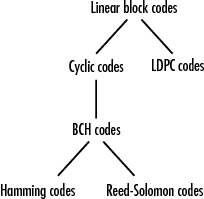
\includegraphics[scale=1]{figuras/blockcodes.png}
      \caption{Uma classifica��o para c�digos de blocos \cite{MathWorks:2010}}
      \label{fig4:cbc}
    \end{figure} 


Um c�digo C � linear se v e w s�o palavras c�digo distintas de um c�digo C, ent�o v+w � tamb�m uma palavra c�digo de C. Um c�digo linear cont�m a palavra c�digo zero, pois $v + v = 0$. Opera��o simples de decodifica��o, pouca mem�ria e m�todos simples para determina��o de padr�es de erros s�o algumas das vantagens de c�digos lineares.

Um c�digo C � chamado de c�clico se o deslocamento c�clico (\emph{shift}) de qualquer palavra c�digo gera uma nova palavra c�digo. Por exemplo, $C1 = \{000, 110, 101, 011\}$   � um c�digo c�clico. $C2 = \{000, 100, 011, 111\}$ n�o � um c�digo c�clico.

\section{C�digos Convolacionais}

P. Elias introduziu c�digos convolucionais em 1955. Um c�digo convulacional � um dispositivo com mem�ria. Apesar de aceitar uma mensagem de entrada de tamanho fixo e produzir uma sa�da codificada, seus c�lculos n�o dependem somente da entrada atual, mas tamb�m das entradas e sa�das anteriores.

Um codificador para um c�digo convolucional tamb�m aceita blocos de $k$ bits da sequ�ncia de dados $u$ e gera uma sequ�ncia de sa�da $v$ de $n$ \emph{bits} chamada \emph{codeword} ou palavra c�digo. Cada bloco da palavra c�digo n�o depende apenas dos $k$ bits do bloco da sequ�ncia de dados correspondente, mas tamb�m de $M$ blocos anteriores. Dizemos que o codificador tem mem�ria de ordem $M$, onde $M$ � o n�mero de registradores de mem�ria. Esse conjunto de blocos de $k$ bits, o codificador das palavras c�digo de tamanho $n$ e de mem�ria de ordem $M$ � chamado de ($n$, $k$, $M$) c�digo convolucional. $R = \frac{k}{n}$  � a taxa de codifica��o. Como o codificador tem mem�ria, ele pode ser implementado como circuito l�gico sequ�ncial \cite{Lin:1983}.

Em um c�digo convolucional, os $n - k$ bits redundantes, que provem � codifica��o a capacidade de tratar os ru�dos do canal, podem ser adicionados quando $k < n$. Para uma mesma taxa de codifica��o $R$, pode-se adicionar redund�ncia, aumentando a ordem da mem�ria $M$ do codificador. Como usar a mem�ria para obter uma transmiss�o confi�vel sob um canal com ru�do � o principal problema do projeto do codificador.

C�digos convolucionais podem ser usados para melhorar o desempenho da comunica��o por r�dio e sat�lites. C�digos convolucionais s�o utilizados nas tecnologias CDMA (\emph{Code division multiple access}) e GSM (\emph{Global System for Mobile Communications}) para telefones celulares, \emph{dial-up modems}, sat�lites, \emph{NASA's Deep Space Network} deep-space communications e na rede WLAN Wi-Fi IEEE 802.11.

\vspace{1cm}

Existem v�rios algoritmos de codifica��o por apagamento \cite{Byers:1998, Kubiatowicz:2000}. Alguns dos mais utilizados s�o c�digos Reed-Solomon (RS), c�digos Low-Density Parity-Check (LDPC) e c�digos Tornado \cite{Mitzenmacher:2004} \cite{RTAD:2007}.

Segundo \cite{Woitaszek:2007}, para sistemas de armazenamento, a codifica��o por apagamento baseada em opera��es simples, tais como XOR RAID e c�digos Tornado,  s�o prefer�veis. Apesar de que um mecanismo externo deva ser utilizado para detectar erros, as opera��es de XOR podem ser realizadas rapidamente e resultar em alto \emph{throughput} das opera��es de codifica��o e decodifica��o.

\section{Caracter�sticas de C�digos de Blocos}

A dist�ncia de Hamming (dH) entre duas palavras c�digo $v_i$ e $v_j$  � o n�mero de \emph{bits} que s�o diferentes nessas duas palavras.

Segundo \cite{AF:2010}, as principais caracter�sticas de c�digos de blocos s�o:

\begin{description}
   \item [taxa de codifica��o] $R = \frac{k}{n}$ � a medida da efici�ncia do c�digo, pois � o quociente do n�mero de \emph{bits} da palavra de dados sobre o n�mero de \emph{bits} total da palavra transmitida
   \item [dist�ncia m�nima] $(d_{min})$ � a menor dist�ncia de Hamming entre duas quaisquer palavras do c�digo; ela depende do n�mero de \emph{bits} redundantes $q = n - k$, tal que  $(d_{min} \leq q + 1)$
   \item [capacidade de detec��o] detecta at� $l$ erros, onde $l \leq d_{min} - 1$
   \item [capacidade de corre��o] corrige os erros at� $t$ erros, onde $ t \leq \lfloor \frac{d_{min} - 1}{2} \rfloor$
   \item [capacidade de detec��o e corre��o] detecta at� $l$ erros e corrige os erros at� $t$ erros, onde $d_{min} \geq l + t + 1$ e $l > t$
\end{description}

Um c�digo com $d_{min} = 1$ n�o tem capacidade de detectar erros.

\section{C�digos de Blocos Lineares}

\subsection{C�digos Reed-Solomon}

S�o c�digos de blocos, lineares e c�clicos.

Definition. A Reed-Solomon (or RS) code over GF(q) is a BCH (BOSE-CHAUDHURI-HOCQUENGHEM) code of length N = q - 1. Of course q is never 2. Thus the length is the number of nonzero elements in the ground field. We shall use N , K and D to denote the length, dimension, and minimum distance (using capital letters to distinguish them from the parameters of the binary codes which will be constructed later). RS codes are important in concatenated codes and burst correction.

Em \cite{Plank:1997}, o autor apresenta uma especifica��o completa do problema e do algoritmo da codifica��o e detalhes de sua implementa��o. O modelo estudado � formado por $n$ dispositivos de armazenamento  $D_1, D_2, ..., D_n$ (\emph{data devices}) e outros $m$ dispositivos de armazenamento  $C_1, C_2, ..., C_m$ (\emph{checksum devices}). O conte�do de cada um dos $m$ \emph{checksum devices} � calculado a partir do conte�do dos $n$ \emph{data devices}. O objetivo do c�lculo dos $C_i$ para $1 \leq i \leq m$ � tal que para quaisquer $m$ dispositivos que falhem dos $D_1, D_2, ..., D_n, C_1, C_2, ..., C_m$, o conte�do dos dispositivos que falharam possa ser reconstitu�do a partir dos dispositivos que n�o falharam.

Segundo \cite{Almeida:2007}, c�digos RS s�o particularmente �teis para corre��o de erros em rajada (seq��ncia s�mbolos consecutivos, nenhum desses recebidos corretamente, chamados \emph{burst errors}). Tamb�m podem ser usados eficientemente em canais onde o conjunto de s�mbolos de entrada � consideravelmente grande.

Uma implementa��o de biblioteca em C/C++ para o algoritmo RS foi apresentada em \cite{Plank:2007}.

O sistema de armazenamento OceanStore \cite{Kubiatowicz:2000} e o protocolo BitTorrent (aplica��o da camada de rede da internet) usam uma codifica��o RS.

\subsection{C�digos RAID}

\emph{Redundant Arrays of Inexpensive [Independent] Disks} (RAID) � uma classe de c�digos RS. RAID � um m�todo para prover toler�ncia a falhas ou alto desempenho em sistemas de armazenagem utilizando para isso uma codifica��o de corre��o de erros ou paridade. RAID foi introduzido por D. A. Patterson na Universidade da California, Berkeley (UC Berkeley) em 1988 \cite{Patterson:1988}.

S�o conceitos b�sicos \cite{Vadala:2002}:

\begin{description}

   \item [data striping] � uma t�cnica para segmentar dados sequ�nciais, como um arquivo, de maneira que o acesso a segmentos sequ�nciais seja feito por diferentes dispositivos de armazenamento. Esta t�cnica � �til quando se quer processar mais rapidamente os pedidos de acesso a dados que os dispositivos de armazenamento permitem. Diferentes segmentos de dados s�o mantidos em diferentes dispositivos de armazenamento. A falha de um dos dispositivos torna toda a sequ�ncia de dados indispon�vel. Essa desvantagem � superada pelo armazenamento de informa��es redundantes (custo de armazenamento extra), como a paridade, com o objetivo de corre��o de erros. As configura��es de RAID que utilizam paridade s�o RAID-2, RAID-3, RAID-4, RAID-5 e RAID-6 \cite{DS:2010}.

   \item [stripe] s�o segmentos consecutivos ou faixas que s�o escritos sequencialmente atrav�s de cada um dos discos de um \emph{array} ou conjunto. Cada segmento tem um tamanho definido em blocos.

\end{description}

\vspace{1cm}

{\bf RAID 2}

\vspace{0.5cm}

Esta configura��o divide os dados a nivel de \emph{bit} e usa c�digos Hamming para corre��o de erros. Por exemplo, o c�digo Hamming(7,4) (quatro \emph{bits} de dados e tres \emph{bits} de paridade) permite usar 7 discos em RAID 2, sendo 4 usados para armazenar dados e 3 usados para corre��o de erros. Esta codifica��o tornou-se padr�o para \emph{hard drives} e tornou-se desnecess�ria, assim deixou de ser vantajosa.

\vspace{1cm}

{\bf RAID 3}

\vspace{0.5cm}

Esta configura��o divide os dados a nivel de \emph{byte} com um disco apenas para paridade. Isto requer que todos os discos operem em \emph{lockstep} (rota��o de todos os discos em sincronismo). Assim como RAID-2, tornou-se obsoleta.

\vspace{1cm}

{\bf RAID 4}

\vspace{0.5cm}

Esta configura��o divide os dados a nivel de bloco com um disco apenas para paridade. Se o controlador de disco permitir, um conjunto RAID 4 pode atender v�rias solicita��es de leitura ao mesmo tempo. Todos os \emph{bits} de paridade est�o em um �nico disco, o que pode se tornar um gargalo. RAID-5 substituiu esta configura��o.

\vspace{1cm}

{\bf RAID 5}

\vspace{0.5cm}

Esta configura��o divide os dados a nivel de bloco com um �nico bloco de paridade por \emph{stripe} e os blocos de paridade ficam distribu�dos por todos os discos. Esta configura��o privilegia a leitura. Uma s�ndrome � computada para permitir a perda de uma unidade. Essa s�ndrome P pode ser um simples XOR de dados pelos \emph{stripes}.

\vspace{1cm}

{\bf RAID 6}

\vspace{0.5cm}

Esta configura��o divide os dados a nivel de bloco com dois blocos de paridade por \emph{stripe} e os blocos de paridade distribu�dos por todos os discos. Duas s�ndromes diferentes precisam ser computadas para permitir a perda de quaisquer duas unidades. Uma delas, P pode ser um simples XOR de dados pelos \emph{stripes}, como em RAID 5. A outra, Q pode ser um XOR de um \emph{linear feedback shift register} de cada \emph{stripe}.

Passo 0: n� 0 cria palavra c�digo em blocos b1, b2, b3, ..., bk

Passo 1: n� 0 cria b1 e o envia para os n� 1 e n� 2

Passo 2: n� 0 cria b2 e o envia para os n� 1 e n� 3

Passo 3: n� 0 cria b3 e o envia para os n� 1 e n� 4

Passo 4: n� 0 e n� 1 codificam b1, b2 e b3 e criam o bloco de paridade p1 = f1(b1, b2, b3) e p2 = f2(b1, b2, b3) 

\vspace{1cm}

\subsection{C�digos Low-Density Parity-Check e Tornado}

S�o c�digos de blocos, lineares e ac�clicos.

C�digo Low-Density Parity-Check (LPDC) �  uma codifica��o baseada em grafos regulares \cite{Gallager:1963}. C�digos LDPC s�o conhecidos tamb�m como c�digos Gallager \cite{LDPCC:2010}. Uma aplica��o dessa codifica��o � a rede \emph{wireless} WMAN WiMAX (IEEE 802.16e \emph{standard for microwave communications}) para internet m�vel \cite{wimax:2010}.

C�digos Tornado s�o uma classe de c�digos LDPC \cite{Woitaszek:2007}. Segundo \cite{Kubiatowicz:2000}, s�o mais r�pidos para codificar e decodificar e necessitam de um pouco mais de $m$ fragmentos para reconstruir a informa��o. 

Em \cite{Luby:1998}, os autores apresentam c�digos Tornado baseados em grafos irregulares. Segundo \cite{CS540:2010}, as implica��es pr�ticas desses c�digos ainda n�o foram bem estudadas.

%Na tabela~\ref{tab1:comp}, alguns sistemas que utilizam com
%codifica��o por apagamento foram comparados.

%
\begin{table}
\singlespacing

  \begin{center}
    \begin{tabular}{|p{2.5cm}||p{2cm}||p{2.7cm}||p{2.5cm}||p{3.5cm}|}
      \hline

Trabalho & Modelo & Objetivos & Codifica��o & M�tricas \\ \hline
Byers,1998 \cite{Byers:1998} & \emph{Digital Fountain} & Confiabilidade, Efici�ncia & Replica��o, c�digos Tornado e RS & tempo de codifica��o e decodifica��o de um bloco \emph{bandwidth}, perda de pacotes\\ \hline

Weatherspoon, 2002 \cite{Weatherspoon:2002:01} & Arquivador central, n�s & Disponibilidade & Replica��o, Codifica��o por Apagamento & tempo m�dio entre falhas, \emph{overhead} de armazenamento, tempo de verifica��o do bloco \\ \hline

Camargo, 2009 \cite{Camargo:2009} & OppStore & Confiabilidade, Disponibilidade & Replica��o  & \emph{bandwidth}, n�mero de mensagens trocadas \\ \hline

Fan, 2009 \cite{Fan:2009}& HDFS & Confiabilidade, Disponibilidade & Replica��o, RAID & atraso na codifica��o do bloco\\ \hline

Dabek, 2004 \cite{Dabek:2004} & DHT & Efici�ncia & Replica��o, Codifica��o por Apagamento & lat�ncia \\ \hline

Houri, 2009 \cite{Houri:2009} & \emph{Peer-to-peer} & Disponibilidade & Replica��o, Codifica��o por Apagamento & \emph{bandwidth} \\ \hline

Plank, 2009 \cite{Plank:2009} & $k$ discos de dados e $m$ discos de paridade & Efici�ncia & c�digos Tornado, RS e RAID & tempo de codifica��o de um grande arquivo de v�deo e tempo de decodifica��o de um \emph{drive} de dados\\ \hline
    \end{tabular}
\caption{Compara��o entre sistemas de codifica��o por apagamento}
\label{tab1:comp}
  \end{center}
\end{table}


%\section{Replica��o versus Codifica��o por Apagamento}

%Para implementar redund�ncia de dados em sistemas, s�o utilizadas v�rias t�cnicas: codifica��o por apagamento, replica��o, espelhamento, \emph{Cyclic redundancy check} (CRC), \emph{bits} de paridade, \emph{checksum}, assinatura digital \cite{EDC:2010}. Mecanismos de redund�ncia podem implementar um conjunto destas t�cnicas \cite{Fan:2009}.

%Entre as t�cnicas para implementar redund�ncia de dados, a replica��o � a mais utilizada em sistemas com o objetivo de se obter alta disponibilidade e durabilidade de dados diante de falhas de componentes destes sistemas. O motivo disto � a simplicidade na implementa��o de replica��o, mas algumas pesquisas demonstram um campo promissor para codifica��o por apagamento para armazenamento em sistemas distribu�dos.

%A principal desvantagem da replica��o � que ela requer um grande \emph{overhead} de armazenamento para pouco ganho em disponibilidade e toler�ncia a falhas. Garantir que os dados permane�am dispon�veis quando todos os $n$ dispositivos falham exige que, pelo menos, $n + 1$ c�pias existam \cite{Woitaszek:2007}. Por exemplo, o sistema Glaciar de armazenamento aumenta de 11 vezes a quantidade de dados armazenados utilizando replica��o para conseguir 0.999999\% (\emph{six nines})  de confiabilidade.

%Uma vantagem de codifica��o por apagamento seria um custo menor de armazenamento se comparado a replica��o, no caso de grande volume de dados. Outra vantagem com rela��o a replica��o foi comentada em \cite{Weatherspoon:2002:01}: para um mesmo espa�o de armazenamento, o tempo m�dio entre falhas (\emph{mean time to failure}) � maior.

%Os autores em \cite{Dabek:2004} afirmam que dados replicados permitem leituras de baixa lat�ncia, porque h� muitas op��es para a sele��o de servidores, enquanto que dados codificados reduzem o consumo de largura de banda para escritas, em detrimento do aumento da lat�ncia de leituras.



   \chapter{Discuss�o sobre esquemas adequados de redund�ncia de dados}

Pode-se encontrar na literatura um n�mero significativo de projetos que prop�em sistemas de armazenamento distribu�do, sistemas de arquivos distribu�dos, ou sistemas de backup. Apesar da disso, nenhum esquema de redund�ncia de dados tem sido amplamente aceito para esses sistemas e nenhuma regra f�cil foi criada para se encontrar um esquema adequado de redund�ncia de dados.

Para implementar redund�ncia de dados em sistemas, s�o utilizadas
v�rias t�cnicas: codifica��o por apagamento, replica��o, espelhamento,
\emph{Cyclic redundancy check} (CRC), \emph{bits} de paridade,
\emph{checksum} e assinatura digital. Esquemas de
redund�ncia podem implementar um conjunto destas
t�cnicas~\cite{Fan:2009}.

Os autores em \cite{Duminoco:2009} estudaram redund�ncia de dados em sistemas \emph{peer-to-peer} para \emph{backup} e propuseram um esquema h�drido para implementar redund�ncia (replica��o e codifica��o) de dados. Em \cite{Storer:2008}, foi proposto um sistema de armazenamento de dados baseado em discos que usa dois n�veis de codifica��o. Nesses textos, encontramos uma compara��o entre alguns sistemas de armazenamento, avaliando-se algumas de suas caracter�sticas. Podemos observar que os tipos de esquema de redund�ncia de dados s�o replica��o, codifica��o por apagamento e h�brido, sendo a replica��o, a estrat�gia mais utilizada nos sistemas comparados por \cite{Duminoco:2009} e a codifica��o por apagamento, para os sistemas comparados por \cite{Storer:2008}.

Redund�ncia de dados � necess�ria para prevenir perda de dados, mas n�o � suficiente. A avalia��o de esquemas de redund�ncia � muitas vezes baseada na suposi��o de que as r�plicas falham de forma independente. Na pr�tica, as falhas n�o s�o t�o independentes, segundo \cite{Weatherspoon:2002:02,Baker:2006}. Esse trabalho n�o tratar� a independ�ncia das r�plicas.

Cada esquema de redund�ncia estabelece (i) como criar os dados redundantes e (ii) como reconstruir os dados quando houver falha. Essas duas opera��es geram custos que diferem de um esquema para outro. Esse trabalho comentar� os mais amplamente usados esquemas de redund�ncia: replica��o e codifica��o por apagamento, que chamaremos de codifica��o.

\section{Esquemas de redund�ncia de dados para sistema de armazenamento}

Esquemas de redund�ncia de dados s�o utilizados em sistemas de armazenamento (exemplo: sistemas RAID) para prover disponibilidade, toler�ncia a falhas e durabilidade de dados e em sistemas de comunica��o (exemplo, sistemas \emph{peer-to-peer}) para prover uma entrega confi�vel e segura de dados.

A Figura~\ref{fig4:srp} apresenta um sistema de armazenamento com um arquivo de dados particionado em 8 blocos. O fator de replica��o � 4. Os clientes precisam que, para cada um dos 8 distintos blocos, uma das quatro c�pias esteja dispon�vel. A Figura~\ref{fig5:crs} apresenta o mesmo sistema que a Figura~\ref{fig4:srp}, mas utilizando c�digos RS. O arquivo est� particionado em 8 blocos e 32 blocos codificados foram gerados. Os clientes podem utilizar quaisquer 8 blocos para obter o arquivo inicial. A Figura~\ref{fig5:crs} tamb�m se aplica a c�digos Tornado.

   \begin{figure}[h]
     \centering
     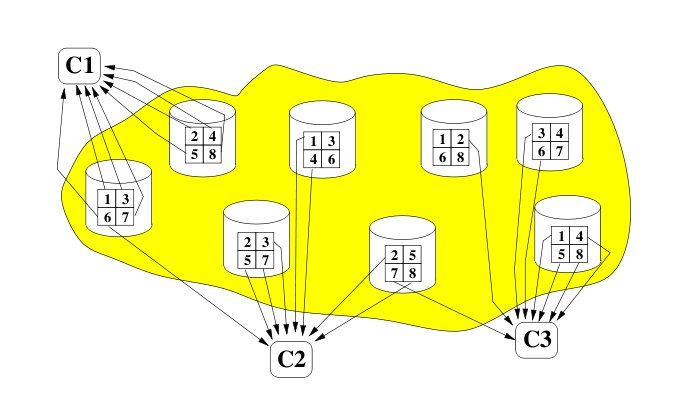
\includegraphics[scale=.6]{figuras/replicacao-pura.jpg}
     \caption{Sistema com replica��o pura \cite{Plank:2004}}
     \label{fig4:srp}
   \end{figure}

   \begin{figure}[h]
     \centering
     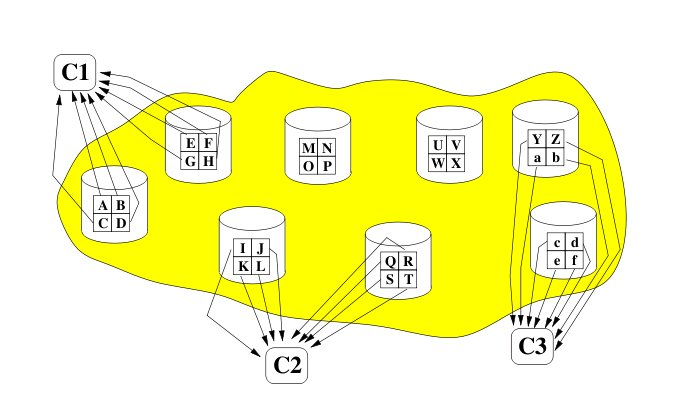
\includegraphics[scale=.6]{figuras/codigos-RS.jpg}
     \caption{Sistema com c�digos RS \cite{Plank:2004}}
     \label{fig5:crs}
   \end{figure}

\subsection{Replica��o}

Replica��o � o esquema de redund�ncia mais simples. A maioria dos sistemas, que utiliza redund�ncia de dados, � baseada em replica��o, mas esse esquema consume mais espa�o que a codifica��o por apagamento, pois uma c�pia completa de cada arquivo � armazenada em cada um dos servidores de dados.

A principal desvantagem da replica��o � que ela requer um grande \emph{overhead} de armazenamento para pouco ganho em disponibilidade e toler�ncia a falhas. Garantir que os dados permane�am dispon�veis quando todos os $n$ dispositivos falham exige que, pelo menos, $n + 1$ c�pias existam \cite{Woitaszek:2007}. Por exemplo, no artigo sobre o sistema Glacier \cite{Haeberlen:2005}, os autores argumentam que o armazenamento aumenta de 11 vezes a quantidade de dados armazenados utilizando apenas replica��o para conseguir 0.999999 (\emph{six nines}) de confiabilidade num cen�rio com 60\% de indisponibilidade dos \emph{peers}.

Os autores em \cite{Dabek:2004} afirmam que dados replicados permitem leituras de baixa lat�ncia, porque h� muitas op��es para a sele��o de servidores, enquanto que dados codificados reduzem o consumo de largura de banda para escritas, em detrimento do aumento da lat�ncia de leituras.

A replica��o � usada no Google File System \cite{Ghemawat:2003} (GFS), no Hadoop Distributed File System \cite{Hadoop:2010} (HDFS) e no Kosmos distributed file system \cite{TKDFS:2011} (KFS), sistemas de arquivos distribu�dos que apresentam caracter�sticas semelhantes. Um \emph{cluster} do GFS ou do HDFS ou do KFS � formado por um �nico servidor, master (GFS) ou namenode (HDFS) ou Meta server (KFS), que mant�m os metadados e muitos servidores de dados, os chunkservers (GFS e KFS) ou os datanodes (HDFS) e � acessado por v�rios clientes. Os arquivos de dados s�o armazenados nos chunkservers (GFS e KFS) ou datanodes (HDFS) e s�o particionados em blocos de igual tamanho. GFS, HDFS e KFS foram projetados para aplica��es que processam grande volume de dados. 

Seus projetos consideram \emph{clusters} de (\emph{commodity hardware}), uma vers�o do \emph{kernel} linux como sistema operacional para as m�quinas e uma arquitetura de rede com dois n�veis: v�rios \emph{racks} interligados por um comutador e cada \emph{rack} � formado por v�rias m�quinas e seus discos, estes tamb�m interligados por um comutador. A estrat�gia de inser��o de dados cria r�plicas em \emph{racks} distintos do \emph{rack} onde est� a 1$^a$ r�plica, assim, falhas que comprometam um \emph{rack} n�o provocam a indisponibilidade de dados. Os arquivos de dados s�o alterados por concatena��es ao inv�s de sobrescrever dados existentes. Ap�s a cria��o, os arquivos de dados s�o usados apenas para leitura e esta leitura ocorre sequencialmente. O KFS permite escrever em posi��es rand�micas nos arquivos. As APIs do cliente fornecidas pelo GFS, pelo HDFS e pelo KFS suportam opera��es de cria��o, leitura, escrita, remo��o de arquivos, mas n�o implementam a interface POSIX.

O GFS est� dispon�vel para linux sob uma licen�a de software propriet�rio. O HDFS \footnote{http://hadoop.apache.org/}  e o KFS \footnote{http://code.google.com/p/kosmosfs/} est�o dispon�veis para linux sob uma licen�a Apache. 

O Farsite, que utiliza apenas replica��o, � um sistema de arquivos distribu�dos, particionados em namespaces, explorando os desktops presentes dentro da Microsoft, sem servidor mestre, dispon�vel para Windows sob uma licen�a de software propriet�rio. A escolha da replica��o foi, pelos autores, considerada uma op��o mais simples para disponibilidade, j� que a codifica��o poderia significar lat�ncia adicional nas leituras dos arquivos. Ainda segundo os autores, estudos com experimentos j� mostraram que a codifica��o pode apresentar um bom desempenho e seria poss�vel, ent�o, alterar no futuro o esquema de redund�ncia do Farsite.

Big Table (constru�do sob o GFS) e Dynamo (constru�do para Amazon.com) s�o dois sistemas de armazenamento que gravam e recuperaram dados atrav�s de uma chave e executam em um \emph{pool} compartilhado de m�quinas, utilizam apenas replica��o. 

Ceph \cite{Weil:2006} � um sistema de arquivos \emph{open source} que possui tr�s principais componentes: um \emph{cluster} de servidores de metadados (que gerencia o namespace, nomes de arquivos e diret�rios), um \emph{cluster} de OSDs (dispositivos de armazenamento de objetos) que armazenam dados e metadados e os clientes que utilizam uma interface do sistema de arquivos. O Ceph agrupa dados em PGs (grupos de coloca��o) e usa uma fun��o \emph{hash} para distribuir os PGs nos OSDs, cujo algoritmo CRUSH � $O(log n)$ e usa uma �rvore-B para indexar os PGs. Existe um m�dulo em desenvolvimento que permite usar o Ceph como armazenamento para uma inst�ncia do Hadoop. O Ceph utiliza apenas replica��o, implementa parcialmente a interface POSIX e est� dispon�vel para linux sob LGPL \footnote{http://ceph.newdream.net/}.

Lustre \footnote{git://git.lustre.org/prime/lustre.git} tem na sua arquitetura os metadata server (disponibiliza os metadados para clientes), o metadata target (um por sistema de arquivos, armazena os metadados), object storage servers (armazena os dados), object storage target (armazena os objetos que cont�m os arquivos de dados) e clientes.

Moosefs \footnote{http://www.moosefs.org/} tamb�m foi projetado com uma arquitetura que se assemelha a do GFS, HDFS e KFS: master server (que armazena os metadados), chunk servers (que armazenam os dados), metalogger server (podem substituir algumas fun��es do master server, se ele falhar) e clientes (que solicitam dados e se comunicam com o master server e o chunk servers. 

Ambos, Lustre e Moosefs, usam replica��o, implementam a interface POSIX e est�o dispon�veis para linux sob uma licen�a GPL.

Com exce��o do Farsite, os sistemas de armazenamento apresentados consideram \emph{clusters} de (\emph{commodity hardware}) e uma vers�o do \emph{kernel} linux como sistema operacional para as m�quinas.

\subsection{Codifica��o por Apagamento}

Uma vantagem de codifica��o por apagamento � um custo menor de armazenamento se comparado a replica��o, no caso de grande volume de dados. Outra vantagem com rela��o a replica��o foi comentada em \cite{Weatherspoon:2002:01}: para um mesmo espa�o de armazenamento, o tempo m�dio entre falhas (\emph{mean time to failure}) � maior.

\begin{table}
%\singlespacing
    \centerline{
    \begin{tabular}{|p{2cm}|p{4cm}|p{5cm}|p{2cm}|}\hline
	{\bf sistema} & {\bf codifica��o} &  {\bf arquitetura do sistema} & {\bf licen�a}\\ \hline
	HDFS \cite{Hadoop:2010}& RAID, RS, ... & shared-disk file system for cluster & Apache\\ \hline
	Tahoe-LAFS \cite{Wilcox-O'Hearn:2008} \footnote{http://tahoe-lafs.org/trac/tahoe-lafs} & RAID & peer-to-peer filesystem & GPL2\\ \hline
	Pergamum \cite{Storer:2008}& XOR parity, RS &  disk-based archival storage & *\\ \hline
	Potshards \cite{Storer:2009} & RAID e RS &  disk-based archival storage & *\\ \hline
	RobuStore \cite{Xia:2006} & Luby Transform (LT) & disk-based archival storage & *\\ \hline
	Glacier \cite{Haeberlen:2005}& RS com matrizes Cauchy & peer-to-peer storage system & *\\ \hline
	Total Recall \cite{Bhagwan:2004} & Maymounkov's online codes &  peer-to-peer storage system & *\\ \hline
	FAB \cite{Saito:2004}& RS & distributed disk array & *\\ \hline
	GPFS \cite{Schmuck:2002}& RAID & shared-disk file system for cluster & *\\ \hline
	Oceanstore \cite{Kubiatowicz:2000} \footnote{http://oceanstore.sourceforge.net/}& Tornado e RS & desktops e notebooks conectados a servidores geograficamente distribu�dos & BSD \\ \hline
	xFS \cite{Anderson:1998} \footnote{http://oss.sgi.com/projects/xfs/} & RAID & serverless network file system & GPL\\ \hline
	Swift \cite{Cabrera:1991} & RAID & desktops sob unix conectados a uma intranet & *\\ \hline
    \end{tabular}}
    \caption{Compara��o de codifica��o entre sistemas de armazenamento de grande volume de dados que utilizam \emph{commodity hardware}}
    \label{tab1:comp}
    onde:\\
    * = n�o dispon�vel
\end{table}


HDFS, Total Recall e OceanStore usam codifica��o para reduzir o tamanho do armazenamento de dados e todos os outros sistemas usam codifica��o para prover disponibilidade e confiabilidade.

Os sistemas que foram comparados na tabela ~\ref{tab1:comp}, est�o dispon�veis para uma vers�o de sistema operacional linux ou unix. Al�m da codifica��o, todos eles implementam replica��o.

Vamos avaliar algumas das m�tricas utilizadas em literatura para comparar redund�ncia de dados em sistemas de armazenamento: sobrecarga de armazenamento, disponibilidade dos \emph{peers}, corrup��o de um dado e opera��es de cria��o, leitura, atualiza��o consistente e remo��o de dados redundantes. Inicialmente vamos definir alguns conceitos adaptados de \cite{Duminoco:2009, Chiola:2005, Rodrigues:2005, Williams:2007} para esses dois esquemas de redund�ncia.

\section{Caracteriza��o da replica��o e da codifica��o}

A confiabilidade de um esquema de redund�ncia � medida pelo n�mero de falhas simult�neas que ele pode tolerar sem comprometer a capacidade de reconstruir os dados originais. Assim esta propriedade pode ser expressada como a {\bf probabilidade de perda de dados, dado que ocorreram $l$ falhas}, $P(l)$.

Para avaliar o armazenamento, vamos definir {\bf fator de redund�ncia} $B$, uma raz�o entre tamanho dos dados originais mais a redund�ncia $|dado\ +\ red|$ e o tamanho dos dados originais $|dado|$ e tamb�m vamos definir grau de repara��o.

O {\bf grau de repara��o} mede o que deve ser feito ap�s parte da redund�ncia ser perdida. Para isso, � feita uma leitura de dados dispon�veis para produzir novos. O custo dessa leitura em um sistema de armazenamento distribu�do inclue volume do tr�fego da rede, pol�tica de repara��o, algoritmo de coordena��o. Nesse estudo vamos apenas avaliar a contribui��o do esquema de redund�ncia: a quantidade de dados a serem lidos para que dados novos sejam criados para reparar o dado corrompido, definido por $d$.

Definimos $p$ como a probabilidade de um \emph{peer} estar dispon�vel e  $q\ =\ 1\ -\ p$ como a probabilidade de um \emph{peer} n�o estar dispon�vel. Nesse estudo, assumimos que elas s�o iguais para todos os \emph{peers}.

Vamos definir as opera��es de acesso a dados redundantes como uma tupla $(r, w, a)$, onde $r$ � o n�mero m�nimo de \emph{peers} dispon�veis que armazenam dados redundantes, $w$ � o n�mero m�nimo de \emph{peers} dispon�veis que armazenam dados redundantes que devem ser acessados para armazenar novos valores e $a$ � n�mero de \emph{peers} (provavelmente outros) que devem estar dispon�veis para completar a opera��o.

\subsection{Replica��o}

Para as defini��es, $n$ � o n�mero de r�plicas dos dados.

{\bf n�mero de falhas suportadas} $l\ =\ n\ -\ 1$

{\bf probabilidade de perda de dados, dado que ocorreram $l$ falhas}

$$
P(l) = \left\{
\begin{array}{rcl}
0,& \mbox{se} & l\ <\ n\\
1,& \mbox{se} & l\ =\ n
\end{array}
\right.
$$

{\bf fator de redund�ncia}
$$
B\ =\ |dado\ +\ red|\ /\ |dado|\ =\ n
$$

{\bf grau de repara��o}
$$
d\ =\ 1
$$

{\bf disponibilidade de um dado}
$$
1 - q^n
$$

{\bf corrup��o de um dado}
$$
e = q^n
$$

\begin{table}
%\singlespacing
    \centerline{
    \begin{tabular}{|p{5cm}|p{5cm}|}\hline
        {\bf acesso} & {\bf tupla $(r, w, a)$}\\ \hline
        criar & $(0, 0, n)$\\ \hline
        apenas leitura & $(1, 0, 0)$\\ \hline
        atualiza��o consistente & $(1, n, 0)$\\ \hline
        apagar & $(0, n, 0)$\\ \hline
    \end{tabular}}
    \caption{Opera��es sobre dados redundantes na replica��o}
    \label{tab2:comp}
\end{table}

Comparando as tuplas (1, 0, 0) e (1, n, 0) da tabela ~\ref{tab2:comp}, podemos observar que a disponibilidade da opera��o "atualiza��o consistente" � menor que a disponibilidade da opera��o "apenas leitura", quando o n�mero de r�plicas $n > 1$ � aplicado.

\subsection{Codifica��o por Apagamento}

Na Codifica��o (m, k), $k$ � o n�mero de blocos originais do dado, $m$ � o n�mero de blocos codificados  e $m\ -\ k$ � o n�mero de blocos adicionados pela codifica��o.

{\bf n�mero de falhas suportadas} $l\ =\ m\ -\ k$

{\bf probabilidade de perda de dados, dado que ocorreram $l$ falhas}
$$
P(l) = \left\{
\begin{array}{rcl}
0,& \mbox{se} & l\ <=\ m\ -\ k\\
1,& \mbox{se} & l\ > m\ -\ k
\end{array}
\right.
$$

{\bf fator de redund�ncia}
$$
B\ =\ m / k
$$

{\bf grau de repara��o}
$$
d\ =\ k
$$

{\bf disponibilidade de um dado}
$$
B(k, m, p)\ =\ \sum_{i=k}^{m}{m \choose i}p^{i}q^{m-i}
$$

{\bf corrup��o de um dado}
$$
e = q^{m-k}
$$

\begin{table}
%\singlespacing
    \centerline{
    \begin{tabular}{|p{5cm}|p{5cm}|}\hline
       {\bf acesso} & {\bf tupla $(r, w, a)$}\\ \hline
       criar & $(0, 0, n)$\\ \hline
       apenas leitura & $(k, 0, 0)$\\ \hline
       atualiza��o consistente & $(k, m-k+1, k-1)$\\ \hline
       apagar & $(0, m-k+1, 0)$\\ \hline
    \end{tabular}}
    \caption{Opera��es sobre dados redundantes na codifica��o por apagamento}
    \label{tab3:comp}
\end{table}

Por outro lado, comparando-se as tuplas $(k, 0, 0)$ e $(k, m-k+1, k-1)$ da tabela ~\ref{tab3:comp}, podemos observar que existe um caso no qual as opera��es "apenas leitura" e "atualiza��o consistente" podem ter a mesma disponibilidade. Isto ocorre quando $m = 2k-1$ (assumindo-se tamb�m que n�mero total de \emph{peers} dispon�veis � maior ou igual a $m$), obtendo-se a tupla $(k, k, k-1)$.


\section{Sobrecarga de armazenamento}

Em \cite{Weatherspoon:2002:01, Dabek:2004}, os autores afirmam que a codifica��o obtem o mesmo n�vel de disponibilidade como a replica��o, usando muito menos espa�o de armazenamento.

Em \cite{Bhagwan:2004}, concluiu-se que se a disponibilidade do peer for 0.5, ent�o isso requer 10 c�pias de cada arquivo para garantir a disponibilidade de 0.999 dos arquivos.

No esquema da replica��o, para um objetivo de probabilidade de indisponibilidade de um dado $e = 0.0001$, dado uma probabilidade de um \emph{peer} estar indispon�vel $q = 0.05$, obtemos o valor de $n = 3$ r�plicas.

$$
\begin{array}{cl}
e\ =\ q^n\\
n\ =\ log\ e\ /\ log\ q\ =\ log\ 0.0001\ / log\ 0.05\ =\ 3.074487147\\
n\ \approx 3
\end{array}
$$

No esquema da codifica��o, para o mesmo objetivo, para as mesmas probabilidades $e$ e $q$, obtemos um valor de 4 blocos de paridade para uma codifica��o $(2k-1, k)$.
 
$$
\begin{array}{cl}
e\ =\ q^{m-k}\\
m\ -\ k\ =\ log\ e\ /\ log\ q
\end{array}
$$

Substituindo $m$ por $2k-1$ e $\ log\ e/\ log\ q$\ por $3.074487147$,
$$
\begin{array}{cl}
k-1\ =\ 3.074487147\\
k\ \approx\ 4 
\end{array}
$$

Para uma mesma probabilidade de indisponibilidade de um dado $e = 0.0001$ e uma mesma probabilidade de um \emph{peer} estar indispon�vel $q = 0.05$, obtemos o valor de $n = 3$ r�plicas para a replica��o e um valor de $k=4$ blocos iniciais para a codifica��o (2k-1,k). O fator de redund�ncia � $B\ =\ 3$ para a replica��o e $B\ =\ m / k\ =\ (2k-1) / k\ =\ 7/4\ =\ 1.75$ para a codifica��o.

No HDFS, a codifica��o RS \emph{default} � (5, 2) e a RAID-5 � (5, 3).  Logo, toleram at� $l=3$ e at� $l=2$ falhas, respectivamente, por \emph{stripe} de 5 blocos ($k=3$) com sobrecarga de $B=2.5$ e de $B=1,6667$, respectivamente.

Nas m�quinas do Facebook, a codifica��o RS � (13, 10) tem 10 blocos iniciais e 3 blocos de paridade ($B=1.3$) e a codifica��o RAID � (12, 10), 10 blocos iniciais e 2 blocos de paridade ($B=1.2$).

Na figura ~\ref{fig1:sarc}, podemos observar o gr�fico \footnote{O gr�fico foi gerado em formato PNG pelo Gnuplot.} das fun��es $y = 2x$, $y = 3x$ e $y = (2x-1)/x$, para $x>0$,  representando a sobrecarga de armazenamento na replica��o $2n$ e na $3n$ e na codifica��o $(2k-1,k)$, respectivamente. O eixo x representa o tamanho de um dado e o eixo y, a sobrecarga de armazenamento desse dado.

    \vspace*{2cm}
    \begin{figure}[h]
      \centering
      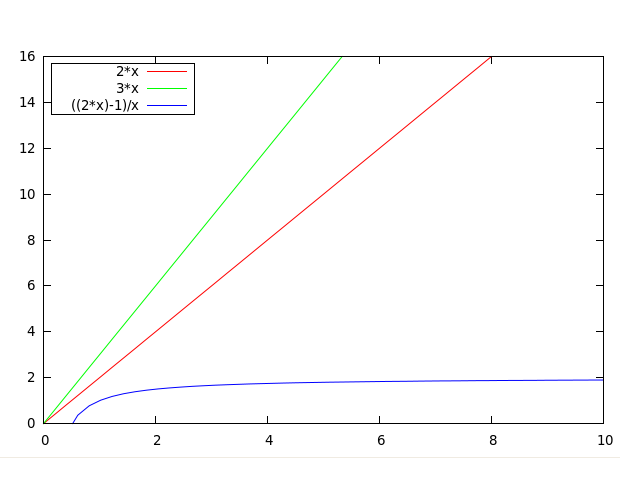
\includegraphics[scale=0.69]{figuras/gnuplot-replicacao-codificacao-3.png}
      \caption{Sobrecarga de armazenamento para replica��o $3n$, $2n$ e codifica��o $(2k-1,k)$ representadas, respectivamente, pelas fun��es $y = 3x$, $y = 2x$ e $y = (2x-1)/x$, para $x>0$}
      \label{fig1:sarc}
    \end{figure}

Neste estudo, conclu�mos que, apenas avaliando a contribui��o do esquema de redund�ncia, a codifica��o por apagamento acarreta uma sobrecarga de armazenamento menor que a replica��o para o mesmo n�mero de falhas toleradas. 

\section{Disponibilidade dos peers}

\section{Leitura ou Atualiza��o dos dados redundantes}

Em \cite{Chiola:2005}, os autores concluem que:

\begin{itemize}
  \item o acesso somente de leitura pode ser suportado tanto por replica��o de dados simples como por codifica��o
  \item para privilegiar atualiza��o consistente, uma codifica��o de alta disponibilidade � necess�ria que se caracteriza por fracionamento do original dados em peda�os $k$ e adicionando exatamente $k-1$ peda�os
  \item se ler e a disponibilidade de atualiza��o consistente s�o de igual import�ncia, isso requer codifica��o $(2k-1, k)$
\end{itemize}

Podemos tamb�m concluir que a replica��o � um caso onde $k = 1$ e $l\ =\ m - k\ = \ n\ -\ 1$, portanto $m\ =\ n$. 

Os autores tamb�m conclu�ram que usar apenas a replica��o tem sentido apenas em poucos casos.



   \chapter{Hadoop}

Atualmente, o Google � uma empresa de consulta e publicidade e � capaz de fornecer os seus servi�os devido a investimentos em armazenamento distribu�do em larga escala e a capacidade de processamento, estes desenvolvidos \emph{in-house}.

Essa capacidade � fornecida por um grande n�mero de PCs, pelo Google File System (GFS), um sistema de arquivos redundantes em \emph{cluster}, pelo sistema operacional GNU/Linux e pelo MapReduce, um \emph{middleware} de processamento paralelo de dados.

Em 2004, um artigo~\cite{Dean:2004}, que foi publicado por
profissionais da Google, prop�s o MapReduce. Em 2006, estes
profissionais, juntamente com Doug Cutting do Yahoo!, formaram um
sub-projeto do Apache Lucene\footnote{http://www.apache.org} que foi
chamado Hadoop\footnote{http://hadoop.apache.org/}.

Mais recentemente, o projeto Apache Hadoop tem desenvolvido uma
reimplementa��o de partes do GFS e MapReduce e muitos grupos da
comunidade de software livre posteriormente abra�aram essa tecnologia,
permitindo-lhes fazer coisas que eles n�o poderiam fazer em m�quinas
individuais. O Hadoop est� dispon�vel em c�digo fonte sob
licenciamento Apache \emph{license} (compat�vel com GPL).

O Hadoop � um \emph{framework} para executar aplica��es em
armazenamento distribu�do de grande volume de dados que pode ser
constru�do com \emph{commodity hardware}, que � facilmente acess�vel e
dispon�vel.  O Hadoop n�o � um \emph{framework} can�nico. Ele foi
projetado para aplica��es que atualizam dados da seguinte forma: uma
escrita e muitas leituras, atrav�s de acessos por \emph{batch}, com
tamanho da ordem de petabytes, organizados de forma n�o estruturada,
com esquema din�mico e integridade baixa.  Uma lista de aplica��es e
organiza��es que usam o Hadoop pode ser encontrada em
\cite{HadoopWiki:2010}.

Em poucas palavras, o Hadoop disponibiliza um armazenamento
compartilhado (HDFS) e um sistema de an�lise (MapReduce) que comp�em o
seu \emph{kernel}.

\section{MapReduce}

O MapReduce utiliza algoritmos de ordena��o para reconstruir sua base de dados.  Um bom uso para o MapReduce s�o aplica��es cujos dados s�o escritos uma vez e lidos muitas vezes. S�o dados n�o estruturados como texto ou imagens. O MapReduce tenta colocar esses dados no n� onde s�o feitas as computa��es, desta forma, o acesso aos dados � r�pido, pois � local \cite{White:2009}.

O MapReduce pode resolver problemas gen�ricos, cujos dados podem ser divididos em matrizes de dados, para cada matriz a mesma computa��o necess�ria (sub-problema) e n�o existe necessidade de comunica��o entre as tarefas (sub-problemas). A execu��o de um t�pico \emph{job} do MapReduce pode ser assim descrita:

\begin{itemize}
    \item Itera��o sobre um n�mero grande de registros
    \item Map extrai algo de cada registro (chave, valor)
    \item Rearranjo (\emph{shuffle}) e ordena��o de resultados intermedi�rios por (chave, valor)
    \item Reduce agrega os resultados intermedi�rios
    \item Gera��o da sa�da
\end{itemize}

Um programas para execu��o no HDFS/MapReduce que podem ser escritos em v�rias linguagens como Java, Ruby, Python e C++.


\section{Arquitetura do Hadoop \emph{Distributed File System}}

Um \emph{cluster} do HDFS � composto por um �nico NameNode, um
servidor-mestre que gerencia o sistema de arquivos e controla o acesso
aos arquivos de clientes. H� uma s�rie de DataNodes, geralmente um por
n� do \emph{cluster}, que gerenciam o armazenamento anexado ao n� em
que s�o executados. A Figura~\ref{fig6:hfs} mostra o NameNode e os
DataNodes.

Uma t�pica arquitetura de rede em dois n�veis para um \emph{cluster}
Hadoop � constru�da por v�rios \emph{racks} interligados por um
comutador como mostra a Figura~\ref{fig5:hc}. Cada \emph{rack} por sua
vez � formado por v�rios n�s (m�quinas) e seus discos, estes tamb�m
interligados por um comutador.

    \vspace*{2cm}
    \begin{figure}[h]
      \centering
      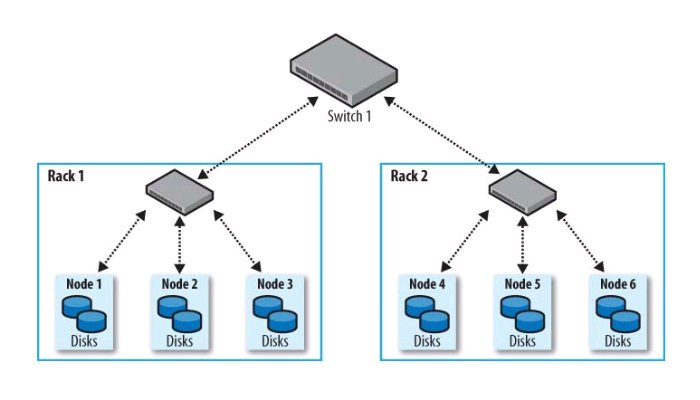
\includegraphics[scale=0.6]{figuras/hadoop-cluster.jpg}
      \caption{Arquitetura de rede em dois n�veis para um cluster Hadoop~\cite{Hadoop:2010}}
      \label{fig5:hc}
    \end{figure} 

O NameNode executa opera��es no sistema de arquivos, como \emph{open}, \emph{close}, \emph{rename} de arquivos e de diret�rios.

HDFS disponibiliza espa�o para sistema de arquivos e permite que os
dados do usu�rio sejam armazenados em arquivos. Internamente, um
arquivo � dividido em um ou mais blocos e esses blocos s�o armazenados
em um conjunto de DataNodes. A Figura~\ref{fig7:hfs} mostra DataNodes
e seus blocos. O tamanho \emph{default} de cada bloco � 64MB.

    \vspace*{2cm}
    \begin{figure}[h]
      \centering
      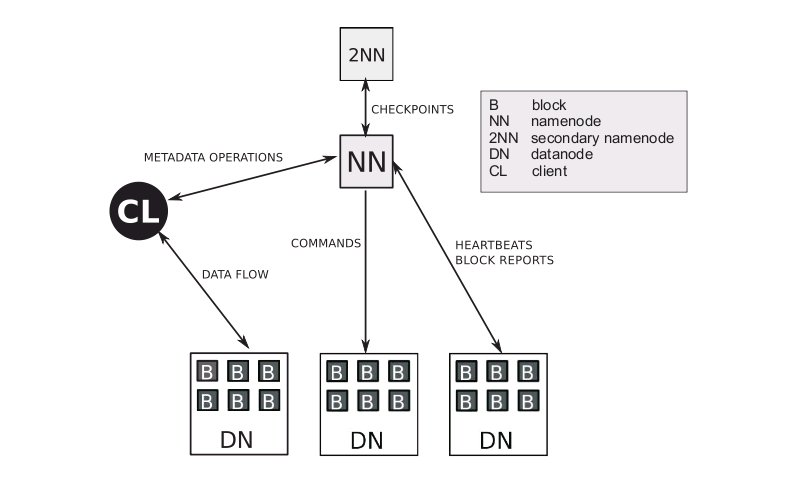
\includegraphics[scale=.6]{figuras/HDFS-arquitetura-2.jpg}
      \caption{Arquitetura do HDFS \cite{TR-IC-10-24}}
      \label{fig6:hfs}
    \end{figure} 

Os DataNodes respondem aos pedidos de leitura e escrita de clientes do
sistema de arquivos e tamb�m executam a cria��o, elimina��o e
replica��o de blocos sob instru��o do NameNode. O n�mero de r�plicas �
geralmente 3. A 1$^a$ r�plica fica local, no mesmo n� do c�digo do
cliente. A 2$^a$ r�plica fica em um n� em outro \emph{rack} e a 3$^a$
r�plica fica nesse �ltimo \emph{rack} em outro n�. As 2$^a$ e 3$^a$
r�plicas n�o s�o locais ao bloco replicado.

O NameNode e DataNode s�o partes do \emph{software} projetado para
rodar em \emph{commodity hardware}. Essas m�quinas normalmente
executam um sistema operacional GNU/Linux.

HDFS � constru�do usando a linguagem Java. Qualquer m�quina que suporte
Java pode executar o NameNode ou o DataNode \cite{Hadoop:2010}.

\vspace*{2cm}
\begin{figure}[h]
  \centering
  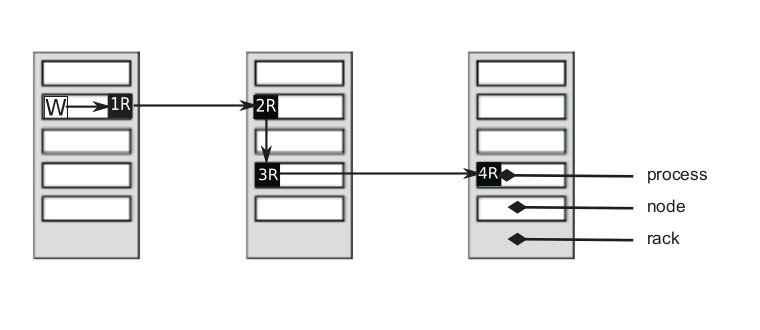
\includegraphics[scale=.5]{figuras/HDFS-arquitetura-replicacao-2.jpg}
  \caption{Arquitetura do HDFS - Datanodes e Blocos \cite{White:2009}}
  \label{fig7:hfs}
\end{figure} 

Os protocolos do HDFS usam o protocolo TCP/IP. O cliente fala o
protocolo ClientProtocol com o NameNode atrav�s de uma porta. Os
DataNodes falam o protocolo DataNodeProtocol com o NameNode. Esses
protocolos executam uma \emph{Remote Procedure Call} (RPC). O NameNode
n�o inicia chamadas RPCs. Ele responde a chamadas RPCs feitas pelo
DataNodes e pelos clientes.

\section{Codifica��o por Apagamento}

Existe uma nova caracter�stica proposta em 2009 para implementa��o de
uma camada de codifica��o por apagamento no Hadoop utilizando
XOR (RAID-5)~\cite{HDFS-503:2010} e uma mais recente utilizando c�digos
RS~\cite{MR-1969:2010}. A inclus�o da codifica��o por apagamento foi proposta com o
objetivo de reduzir o tamanho do armazenamento do HDFS.

A vers�o atual do Hadoop n�o utiliza apenas a t�cnica de replica��o
\cite{White:2009} para obter disponibilidade e confiabilidade de
dados. Ela pode ser configurada para usar tamb�m  codica��o XOR (RAID-5) e RS.

No HDFS, a codifica��o RS \emph{default} � (8, 5) e a XOR \emph{default} � (6, 5).  Logo, toleram at� $l=3$ e at� $l=1$ falhas, respectivamente, por \emph{stripe} de 5 blocos ($k=5$) com sobrecarga de $B=1.6$ e de $B=1.2$, respectivamente.

Na codifica��o XOR, � poss�vel configurar o n�mero de blocos por \emph{stripe}. J� na codifica��o RS, tanto o n�mero de blocos por \emph{stripe} e como o n�mero de blocos de paridade s�o configur�veis.

\subsection{Algoritmos da Camada RAID}

Exemplo do algoritmo de codifica��o

O tamanho da \emph{stripe} � 5 blocos e existe um arquivo $/a/arquivo.txt$ com exatamente 5 blocos. Nesse caso, o algoritmo de codifica��o da camada RAID faz o seguinte:

\begin{verbatim}
bloco[0] = primeiro bloco
bloco[1] = segundo bloco
bloco[2] = terceiro bloco
bloco[3] = quarto bloco
bloco[4] = quinto bloco

bloco_paridade = iniciado com 0 em todos os bytes

para i de 0 at� n�mero de bytes em um bloco:
   para j de 0 at� 4:
      bloco_paridade = bloco_paridade xor bloco[j][i]

para i de 0 at� 4:
   escreva bloco_paridade no arquivo /raid/a/arquivo.txt
\end{verbatim}

\subsection{Algoritmos da Camada RS}

Exemplo do algoritmo de codifica��o

O tamanho da \emph{stripe} � 5 blocos, s�o 3 blocos de paridade, o polin�mio primitivo � $x^8 + x^4 + x^3 + x^2 + 1$ e existe um arquivo $/a/arquivo.txt$ com exatamente 5 blocos. Nesse caso, o algoritmo de codifica��o da camada RS faz o seguinte:

\begin{verbatim}
// polin�mio primitivo g representado por 285
g = x^8 + x^4 + x^2 + x + 1 
m = 8
k = 5
i = 0
L = m-k
j = 0

bloco[0] = primeiro bloco
bloco[1] = segundo bloco
bloco[2] = terceiro bloco
bloco[3] = quarto bloco
bloco[4] = quinto bloco

enquanto j >= L fa�a
   // para GF = 2
   // x^0 representado por 1; x^1 por 2; x^2 por 4; x^3 por 8; 
   // x^4 por 16; x^5 por 32; x^6 por 64; x^7 por 128;
   a = x^j
   i = 0
   bloco_paridade[j] = iniciado com 0 em todos os bytes
   enquanto i >= k fa�a
      r = novo bloco
      resto(g, a, bloco[i], r)
      bloco_paridade[j] = bloco_paridade[j] xor r
      i++
   j++
   
para j de 0 at� L
   escreva bloco_paridade[j] no arquivo /raidrs/a/arquivo.txt

resto (g, a , bloco, r)
   para i de 0 at� n�mero de bytes em um bloco:
      r[i] = resto(g, a, bloco[i])

resto (g, a, b)
retorna resto = (byte) rem (g(b), a(b))
   
\end{verbatim}


    \bibliographystyle{plain}
    \bibliography{referencias/ref-dissertacao}
    \end{document}
